\chapter{RDF}

\begin{definition}{RDF}

    RDF (Resource Description Framework) è uno standard per rappresentare
    informazioni e relazioni tra risorse attraverso triple:

    \begin{center}
        $(soggetto, predicato, oggetto)$
    \end{center}

    Ogni tripla è detta \textbf{statement}.

\end{definition}

Dove:

\begin{itemize}

    \item \textbf{Soggetto}: è la risorsa di cui si parla
    nell'informazione.

    \item \textbf{Predicato}: rappresenta una proprietà o una relazione
    tra il soggetto e l'oggetto.

    \item \textbf{Oggetto}: è la risorsa o il valore a cui si riferisce
    la proprietà.

\end{itemize}

In RDF si introducono due concetti importanti: quello di URI e quello
di risorsa.

\begin{definition}{URI}

    Un URI è una stringa che identifica una risorsa.

\end{definition}

\begin{definition}{Risorsa}

    Una risorsa è qualsiasi entità che può essere identificata e descritta
    mediante un identificatore, come un URI.

    Può rappresentare, ad esempio:

    \begin{itemize}
        \item una cosa del mondo reale;
        \item una proprietà o una relazione;
        \item un'entità astratta.
    \end{itemize}

\end{definition}

\begin{center}
    L'idea di base di RDF è quella di identificare e descrivere le risorse
    mediante opportuni identificatori, in particolare URI/IRI.
\end{center}

\begin{observation}{Grafo RDF}

    L'insieme delle triple RDF può essere rappresentato come un
    \textbf{grafo diretto etichettato}: le risorse rappresentano i nodi,
    mentre i predicati rappresentano gli archi, orientati dal soggetto
    verso l'oggetto.

    Questo permette di concatenare più triple, utilizzando l'oggetto
    di una tripla come soggetto di un'altra.

\end{observation}
\newpage


Quindi a questo punto, soggetto predicato e oggetto, sono tutte delle risorse, cioè \textbf{degli URI}.


Il fatto è che io vorrei anche non avere solo risorse in RDF, ma vorrei esprimere anche \textbf{Interi,Booleani,Stringhe\dots}


A questo ci servono i Literal:

\section{Literal}



\begin{definition}{Literal}
    Un literal rappresenta un valore concreto, come:
    \begin{itemize}
        \item "Diego Maradona"
        \item "Argentina"
        \item  123
        \item 30-10-1960
    \end{itemize}
\end{definition}
\begin{warning}{Literal $\neq$ Risorsa}
Un literal non è una risorsa, una risorsa è una qualunque cosa identificabile tramite un URI.
\end{warning}

I litterali possono essere di due tipi:
\begin{itemize}
    \item tipati.
    \item non tipati.
\end{itemize}
\begin{figure}[htbp]
    \centering
    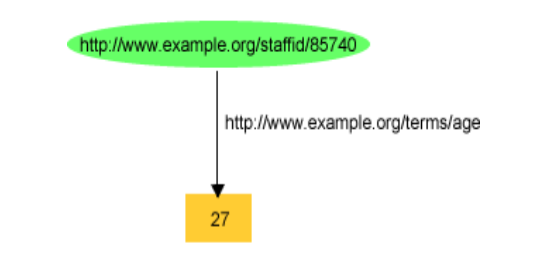
\includegraphics[width=0.7\textwidth]{_files/_images/rdf1.png}
    \caption{Risorsa collegata ad un Literal Non tipato}
    \label{fig:etichetta}
\end{figure}
In questo caso, 27 è non tipato, perchè non stiamo specificando il suo tipo.

\newpage    

\begin{definition}{Letterale Tipato}
    Un litterale tipato è formato da una stringa,e un URI, \textbf{che ne specifica il tipo}.

    La sintassi è la seguente:
    \begin{center}
        \texttt{stringa\string^\string^URIref}
    \end{center}
    dove URIref, è l'uri del datatype, del valore nella stringa, che ne specifica il tipo.
\end{definition}

\begin{example}{Esempio di letterale tipato}
    \texttt{"27"\string^\string^http://www.w3.org/2001/XMLSchema\#integer}
\end{example}

RDF non definisce un insieme di datatype, esistono definiti quindi esternamente a RDF, tipicamente, RDF prende i datatype da XML Schema.


Il datatype, è formato da 3 parti principali:
\begin{itemize}
    \item \textbf{Value Space} : È l'insieme dei valori effettivi che appartengono a quel tipo.
    Per xsd::integer è
    \begin{lstlisting}
        ..., -2, -1, 0, 1, 2, 3, ..., 42, ... 
    \end{lstlisting}
    questi rappresentano i valori di quel tipo
    \item \textbf{Lexical space}
    È l'insieme delle stringhe ammesse per rappresentare quei valori.
    Per esempio, per il valore 42, si ha:
    \begin{itemize}
        \item "42"
        \item "+42"
    \end{itemize}
    \item \textbf{Lexical-to-value mapping} : Questa è semplicemente la funzione che dice:
    \begin{center}
        "Questa stringa, quale valore rappresenta?"
    \end{center}
    Quindi collega, il valuespace al lexical space, è il ponte fra i due spazi.
    Per esempio:
    \begin{lstlisting}
        "42"  --------->  42
        "+42" --------->  42
    \end{lstlisting}
\end{itemize}
\begin{center}
    \textbf{I literal, possono comparire solo come oggetti.Quindi nella tripla, sono comparire solo come terzo elemento}
\end{center}
Quindi facendo il punto della situazione,per ora con RDF possiamo rappresentare, risorse (che sono identificate da un URI) e letterali.


Le triple per ora, saranno qualcosa del genere:
\begin{example}{Esempio Triple in RDF}

Consideriamo la seguente informazione:

\begin{center}
\textbf{Diego Maradona ha come data di nascita il 30-10-1960.}
\end{center}

Possiamo rappresentarla tramite la seguente tripla RDF:

\begin{center}
\texttt{(Maradona, dataDiNascita, "30-10-1960")}
\end{center}

dove:

\begin{itemize}
\item \texttt{Maradona} è il \textbf{soggetto}, cioè una risorsa identificata tramite un URI;
\item \texttt{dataDiNascita} è il \textbf{predicato}, anch'esso identificato tramite un URI;
\item \texttt{"30-10-1960"} è l'\textbf{oggetto}, che in questo caso è un literal, non tipato, e quindi lo si interpreta come una stringa.
\end{itemize}

Quindi una tripla RDF può avere come oggetto sia una \textbf{risorsa} sia un \textbf{literal}.

Ad esempio:

\begin{center}
\texttt{(Maradona, giocaPer, SSC Napoli)}
\end{center}

ha come oggetto una \textbf{risorsa}, mentre:

\begin{center}
\texttt{(Maradona, numeroMaglia, "10"\string^\string^\texttt{http://www.w3.org/2001/XMLSchema\#integer})}
\end{center}

ha come oggetto un \textbf{literal tipato}.
\end{example}

\begin{center}
Quindi in RDF, per ora, le triple sono formate da URI (soggetto, predicato, oggetto) e,limitatamente alla posizione di oggetto, da letterali.    
\end{center}

\begin{definition}{Modello dei Dati RDF}
    RDF (parliamo di RDF base senza serializzazioni, quindi come modello dei dati) definisce un modello di dati astratto basato su un insieme di triple:
    \begin{center}
        (s,p,o)
    \end{center}
    Dove:
    \begin{itemize}
        \item \textbf{s} = soggetto.
        \item \textbf{p} = predicato.
        \item \textbf{o} = oggetto.
    \end{itemize}
    Dove il soggetto può essere una risorsa,o un blank node, il predicato deve essere una risorsa, e l'oggetto può essere una risorsa,literal o blank node.
\end{definition}


\newpage

\section{Blank Nodes}
Per ora abbiamo introdotto:
\begin{itemize}
    \item \textbf{Risorse} : che sono identificate da URI.
    \item \textbf{Literal} : che sono valori letterali, che sono tipati o non tipati.
\end{itemize}
Ora consideriamo il seguente esempio:
\begin{center}
    exstaff:85740 exterms:address "1501 Grant Avenue, Bedford, Massachusetts 01730" . \footnote{Questa è una serializzazione Turtle, l'abbiamo scritto solo per comodità ma in realtà stiamo ancora in RDF standard e quindi URI completi.}
\end{center}
L'indirizzo è rappresentato come una unica stringa, in genere però conviene suddividerlo in
parti (via, città, stato, codice postale) ottenendo così una informazione aggregata.

Per esempio , quello che si può fare è:
\begin{lstlisting}
exstaff:85740 exterms:address exaddressid:85740 .
exaddressid:85740 exterms:street "1501 Grant Avenue" .
exaddressid:85740 exterms:city "Bedford" .
exaddressid:85740 exterms:state "Massachusetts" .
exaddressid:85740 exterms:postalCode "01730" .
\end{lstlisting}
\begin{figure}[htbp]
    \centering
    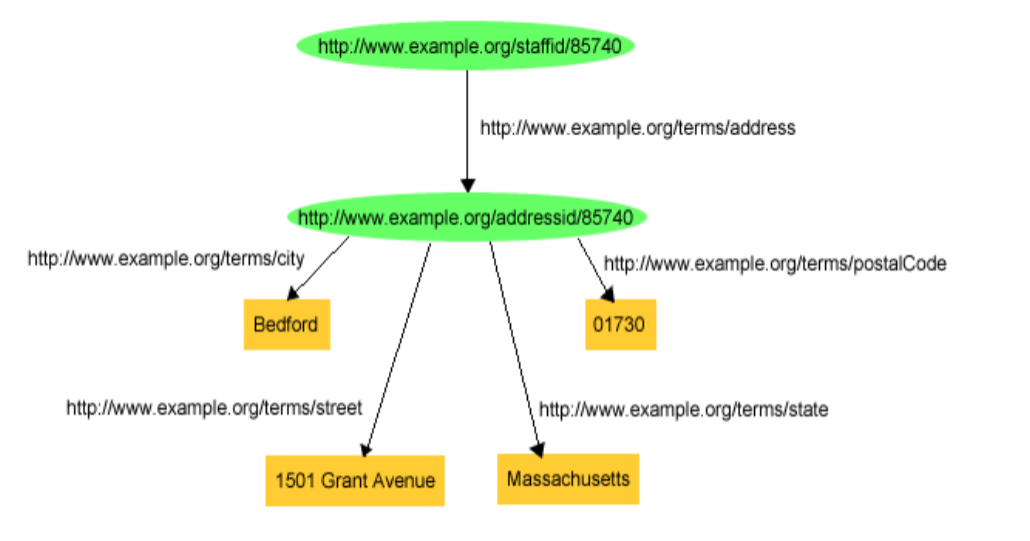
\includegraphics[width=0.7\textwidth]{_files/_images/rdf2.png}
    \caption{Rappresentazione a grafo, del codice turtle sopra}
    \label{fig:etichetta}
\end{figure}
\begin{warning}{Problema}
In questo modo però si generano numerosi URIref di servizio , come ad esempio
exaddressid:85740 per reificare informazioni aggregate. Tuttavia
dall'esterno nessuno può voler riferirsi direttamente a queste reificazioni per questo
non sembra che meritino degli identificatori universali come gli URIref
\end{warning}
Per questo motivo RDF consente di usare in questi casi dei blank node.
\begin{definition}{Blank Node}
    Un blank node è un nodo con una etichetta anonima (ovvero non associata a nessun URI).

    Un blank node viene rappresentato in RDF standard, in questo modo:
    \begin{center}
        \texttt{\_:identificativo}
    \end{center}
\end{definition}
L'identificativo del Blank Node (come \texttt{\_:b1} o \texttt{\_:node123}) è un puro artificio locale: ha valore soltanto all'interno di quel determinato documento o modello RDF.
\begin{itemize}
    \item  Non è un identificativo globale: Fuori da quel modello RDF specifico, l'ID del Blank Node non esiste. Non puoi usarlo come indirizzo sul Web.
    Invece l'URI è un identificativo globale.
    \item Non puoi fare un lookup diretto: Non potendo digitare una richiesta web diretta per quello specifico Blank Node, non puoi interrogarlo isolatamente per dire ``Web, dammi le informazioni sul nodo \texttt{\_:\allowbreak b1}.''
\end{itemize}
\textbf{Un blank node può occorrere come soggetto o oggetto di una tripla, non come
predicato}

Quindi questi sono i principali pezzi del RDF standard, le risorse, i blank node e i literal.



\section{URI e URL}
L'URI è lo standard generale per denotare qualsiasi risorsa, reale o astratta.
Gli URIs(a differenza degli URL) non si limitano a denotare risorse che sono deferenziabili sul Web,
ovvero che hanno una locazione sulla rete.

\begin{definition}{URL}
    L'URL è una stringa che identifica la posizione di una risorsa e permette di accedervi, \textbf{questo implica}
    che l'URI ha un \textbf{meccanismo di accesso (http, ftp, ecc.), che permette di recuperare effettivamente la risorsa in rete}.

    Quindi se prendo un URL e lo "cerco" (cioè lo dereferenzi, ad esempio digitandolo nel browser),
    il sistema sa esattamente dove andare a bussare e — se tutto funziona correttamente — ottieni indietro la risorsa stessa (una pagina HTML, un'immagine, un file...).

    Con l'URI generico questo non è garantito.
\end{definition}

\textbf{Quindi l'URL è un URI che identifica anche dove e come cercare la risorsa.}

Gli URI possono identificare invece anche risorse non deferenziabili, cioè che \textbf{non ha nessuna locazione di rete associata}, 
ad esempio una persona, un concetto astratto, una proprietà.



RDF usa gli URI, perchè se ne infischia della deferenziabilità, basta identificare le risorse insomma, mentre ad esempio il browser,\textbf{assume}
che io gli stia dando un URL, quindi tenta sempre di dereferenziarlo per restituirti un contenuto, nel caso di alcuni URI, ovviamente questa 
deferenziazione non va a buon fine, per quello detto prima.

\subsection{URI schemes}
Ci sono diversi schemi di URI che sono usati per vari scopi, per identificare risorse in modo differente:
\begin{itemize}
    \item \textbf{http} : HypertextTransfer Protocol, per denotare la locazione di pagine Web. (In questo caso è anche un URL)
    \item \textbf{mailto} : indirizzi email, e.g., mailto:em@w3.org
    \item \textbf{ftp} : FileTransfer Protocol.
\end{itemize}
\section{URIrefs}
\begin{definition}{URIrefs}
    URIrefs = URI + frammento identificativo
\end{definition}
\begin{example}{URIrefs}
    http://www.example.org/index.html\#section2

    \begin{itemize}
        \item è formato da un URI (http://www.example.org/index.html), che è la risorsa, cioè la pagina.
        \item e un frammento identificativo : \#section2 ad esempio una parte specifica dentro quella pagina.
    \end{itemize}
\end{example}
Gli URIrefs possono essere assoluti o relativi.

\begin{example}{URIrefs relativo}
    URIref relativo \#section2 quando occorre nella risorsa http://www.example.org/index.html 
    viene completato ottenendo URIref assoluto http://www.example.org/index.html\#section2
\end{example}

\begin{observation}{URIrefs in HTML vs RDF}
    Una differenza sostanziale fra come gli URIrefs sono usati in HTML e RDF è laseguente. 
    Si consideri per esempio gli URIrefs:
    \begin{itemize}
        \item http://www.example.org/index.html
        \item http://www.example.org/index.html\#Section2
    \end{itemize}
    Nell'uso abituale di HTML, questi URIrefs sono correlati: entrambi si riferiscono allo stesso documento, 
    in particolare il secondo identifica una locazione all'interno del primo.


    RDF invece non fa nessuna particolare assunzione, i due riferimenti sono per RDF
    completamente irrelati. Essendo URIrefsintatticamente differenti possono riferirsi a
    risorse completamente diverse. 
\end{observation}
\section{Serializzazioni}

Finora abbiamo parlato di \textbf{RDF come modello di dati}, ovvero come un insieme di triple della forma

$$
(soggetto,\ predicato,\ oggetto)
$$

dove soggetto, predicato e oggetto possono essere risorse identificate tramite URI, mentre l'oggetto può essere anche un \textbf{literal} o un \textbf{blank node}, mentre il soggetto può essere anche un blank node.

Una serializzazione è una particolare sintassi che permette di trasformare il modello RDF in una rappresentazione testuale o, più in generale, in un formato memorizzabile e scambiabile.

Esistono diverse serializzazioni RDF, tra cui:

\begin{itemize}
\item \textbf{Turtle}: sintassi compatta e leggibile, che permette di utilizzare prefissi e abbreviazioni;
\item \textbf{RDF/XML}: serializzazione di RDF basata sulla sintassi XML;
\item \textbf{JSON-LD}: serializzazione basata su JSON, particolarmente adatta allo scambio di dati sul Web;
\item \textbf{N-Triples}: serializzazione molto semplice, in cui ogni tripla viene rappresentata esplicitamente;
\item \textbf{N-Quads}: estensione di N-Triples che permette di rappresentare anche più grafi RDF.
\end{itemize}

Le diverse serializzazioni \textbf{non definiscono modelli RDF differenti}: rappresentano lo stesso modello di dati attraverso sintassi differenti.

Ad esempio, la stessa informazione RDF

\[
\left(
\texttt{http://example.org/Mario},
\texttt{http://xmlns.com/foaf/0.1/name},
\texttt{"Mario"}
\right)
\]

può essere rappresentata in Turtle come:

\begin{verbatim}
@prefix ex: <http://example.org/> .
@prefix foaf: <http://xmlns.com/foaf/0.1/> .

ex:Mario foaf:name "Mario" .
\end{verbatim}

oppure in N-Triples come:

\begin{verbatim}
<http://example.org/Mario>
<http://xmlns.com/foaf/0.1/name>
"Mario" .
\end{verbatim}

Le due rappresentazioni hanno \textbf{lo stesso significato a livello del modello RDF}; cambia solamente la sintassi utilizzata per serializzarlo.

In particolare, elementi come \textbf{prefissi, QNames e abbreviazioni sintattiche} non fanno parte del modello RDF astratto, ma sono caratteristiche offerte da alcune specifiche serializzazioni. Ad esempio, il QName

$$
\texttt{foaf:name}
$$

è una forma abbreviata utilizzabile in Turtle, ma il modello RDF considera comunque l'URI completo:

$$
\texttt{http://xmlns.com/foaf/0.1/name}.
$$


Il \textbf{modello RDF} definisce la struttura e il significato dei dati, mentre la \textbf{serializzazione} definisce come tali dati vengono concretamente rappresentati e scritti.

\begin{center}
    \textbf{Le serializzazioni definiscono come rappresentare il modello RDF astratto in un testo/file.}    
\end{center}

Le serializzazioni RDF sono sintassi concrete utilizzate per rappresentare in un documento testuale il modello RDF astratto.


\section{N-Triples}

N-Triples è una sintassi di serializzazione per RDF che permette di rappresentare le triple RDF in una forma semplice, esplicita e non ambigua.

Ogni tripla viene rappresentata separatamente nella forma:

\begin{center}
\texttt{soggetto predicato oggetto .}
\end{center}

Una tripla può contenere:

\begin{itemize}

\item un URI come soggetto, predicato o oggetto;
\item un \textit{blank node} come soggetto o oggetto;
\item un literal come oggetto.

\end{itemize}

Ad esempio:

\begin{center}
\texttt{<http://example.org/Andrew> <http://xmlns.com/foaf/0.1/knows> <http://example.org/Matt> .}
\end{center}
\textbf{Gli URI in N-triples, sono racchiusi fra parentesi angolate} : <URI> \\
\textbf{I literal in N-triples, sono rappresentati cosi : ``valore''\textasciicircum\textasciicircum<URI-datatype>}

\subsection*{Regole principali}

N-Triples non utilizza abbreviazioni sintattiche. Ogni tripla deve essere scritta esplicitamente e terminata dal punto (\texttt{.}).

Ad esempio, se un soggetto è associato a più proprietà:

\begin{center}
\texttt{<http://example.org/Andrew> <http://xmlns.com/foaf/0.1/knows> <http://example.org/Matt> .} 

\texttt{<http://example.org/Andrew> <http://xmlns.com/foaf/0.1/surname> "Perez-Lopez" .}

\end{center}

il soggetto deve essere ripetuto in entrambe le triple.

Analogamente, se uno stesso soggetto e predicato sono associati a più oggetti, ogni tripla deve essere scritta separatamente:

\begin{center}
\texttt{<http://example.org/Andrew> <http://xmlns.com/foaf/0.1/knows> <http://example.org/Matt> .}


\texttt{<http://example.org/Andrew> <http://xmlns.com/foaf/0.1/knows> <http://example.org/Ryan> .}

\texttt{<http://example.org/Andrew> <http://xmlns.com/foaf/0.1/knows> <http://example.org/John> .}


\end{center}

Quindi, N-Triples privilegia una rappresentazione \textbf{esplicita delle singole triple}, senza introdurre abbreviazioni per raggruppare più triple.

\section{Turtle}

Turtle (\textit{Terse RDF Triple Language}) è una sintassi di serializzazione per RDF che permette di rappresentare le triple RDF in una forma più \textbf{compatta e leggibile}.

A differenza di N-Triples, Turtle permette di utilizzare diverse \textbf{abbreviazioni sintattiche}, che consentono di evitare la ripetizione di parti comuni delle triple.

\subsection*{@prefix}

Una delle principali abbreviazioni consiste nell'utilizzo dei \textbf{prefissi}, che permettono di sostituire una parte comune degli URI con un identificatore più breve.

Ad esempio:

\begin{center}
\texttt{@prefix foaf: <http://xmlns.com/foaf/0.1/> .}
\end{center}

Dopo aver definito il prefisso, è possibile scrivere:

\begin{center}
\texttt{foaf:name}
\end{center}

invece dell'URI completo:

\begin{center}
\texttt{<http://xmlns.com/foaf/0.1/name>}
\end{center}

Analogamente, possiamo definire:

\begin{center}
\texttt{@prefix people: <http://example.org/people/> .}
\end{center}

e utilizzare \texttt{people:Andrew} al posto dell'URI completo.

\subsection*{@base}

La direttiva \texttt{@base} permette di specificare una \textbf{base URI} all'interno di un documento Turtle.

Viene utilizzata per poter scrivere delle URI in forma \textbf{relativa}, evitando di dover ripetere ogni volta la parte comune della URI.

La sintassi è:
\[
\texttt{@base <URI-base> .}
\]

Ad esempio:
\begin{verbatim}
@base <http://example.org/> .

<student/123> <name> "Giuliano" .
\end{verbatim}

La URI relativa \texttt{<student/123>} viene risolta rispetto alla base URI:
\[
\texttt{http://example.org/student/123}
\]

Analogamente:
\begin{verbatim}
@base <http://example.org/data/> .

<student/123>
\end{verbatim}

corrisponde a:
\[
\texttt{http://example.org/data/student/123}
\]

\paragraph{Scopo}
\texttt{@base} serve quindi a:
\begin{itemize}
    \item definire una URI di riferimento per il documento;
    \item permettere l'utilizzo di URI relative;
    \item rendere il documento più compatto e leggibile.
\end{itemize}

\paragraph{Attenzione}
\texttt{@base} riguarda la \textbf{risoluzione delle URI relative} e non definisce un prefisso.

Ad esempio:

\begin{verbatim}
@base <http://example.org/> .
@prefix ex: <http://example.com/> .
\end{verbatim}

hanno due scopi differenti:
\begin{itemize}
    \item \texttt{@base} stabilisce la base per risolvere URI relative;
    \item \texttt{@prefix} associa un prefisso ad uno spazio di nomi, permettendo di utilizzare URI abbreviate come \texttt{ex:Student}.
\end{itemize}



\subsection*{Statement semplice}

Uno statement semplice ha la forma:

\begin{center}
\texttt{people:Ryan ext:worksWith people:John .}
\end{center}

che rappresenta direttamente una tripla RDF.

\subsection*{Abbreviazione tramite punto e virgola}

Più statement che condividono lo stesso soggetto possono essere scritti in forma sintetica, specificando il soggetto una sola volta e utilizzando il punto e virgola (\texttt{;}) tra i diversi predicati.

\begin{center}
\texttt{people:Andrew foaf:knows people:Matt ;}\
\texttt{\phantom{people:Andrew }foaf:surname "Perez-Lopez" .}
\end{center}

Questa forma è equivalente alle due triple:

\begin{center}
\texttt{people:Andrew foaf:knows people:Matt .}\
\texttt{people:Andrew foaf:surname "Perez-Lopez" .}
\end{center}

Il punto e virgola, quindi, permette di \textbf{non ripetere il soggetto}.

\subsection*{Abbreviazione tramite virgola}

Più statement che condividono lo stesso soggetto e predicato possono essere raggruppati utilizzando la virgola (\texttt{,}).

\begin{center}
\texttt{people:Andrew foaf:knows people:Matt , people:Ryan , people:John .}
\end{center}

Questa forma è equivalente alle tre triple:

\begin{center}
\texttt{people:Andrew foaf:knows people:Matt .}\
\texttt{people:Andrew foaf:knows people:Ryan .}\
\texttt{people:Andrew foaf:knows people:John .}
\end{center}

La virgola, quindi, permette di \textbf{non ripetere né il soggetto né il predicato}.

\subsection*{Confronto con N-Triples}

Le abbreviazioni di Turtle non modificano il significato delle informazioni rappresentate: permettono semplicemente di scrivere in maniera più compatta le stesse triple RDF.

Ad esempio, le tre triple:

\begin{center}
\texttt{people:Andrew foaf:knows people:Matt .}\
\texttt{people:Andrew foaf:knows people:Ryan .}\
\texttt{people:Andrew foaf:knows people:John .}
\end{center}

possono essere abbreviate in Turtle come:

\begin{center}
\texttt{people:Andrew foaf:knows people:Matt , people:Ryan , people:John .}
\end{center}

Pertanto:

\begin{center}
\textbf{RDF} $\rightarrow$ modello astratto basato su triple
\end{center}

\begin{center}
\textbf{N-Triples / Turtle} $\rightarrow$ sintassi per serializzare tali triple
\end{center}

N-Triples privilegia la semplicità e l'esplicitazione delle triple, mentre Turtle introduce abbreviazioni che rendono la rappresentazione più compatta e leggibile.



\subsection{Blank Node}

I blank node possono essere espressi utilizzando dei riferimenti anonimi \texttt{\_:x} oppure attraverso una forma compatta mediante parentesi quadre \texttt{[,]}.

\vspace{1em}

\noindent
\begin{minipage}[t]{0.48\textwidth}
\textbf{Uso di riferimenti anonimi (\texttt{\_:abc}):}
\begin{lstlisting}
@prefix rdf: <http://www.w3.org/1999/02/22-rdf-syntax-ns#>.
@prefix dc: <http://purl.org/dc/elements/1.1/>.
@prefix exterms: <http://www.example.org/terms/>.

<http://www.w3.org/TR/rdf-syntax-grammar>
    dc:title "RDF/XML Syntax Specification (Revised)" ;
    exterms:editor _:abc .

_:abc
    exterms:fullName "Dave Beckett" ;
    exterms:homePage <http://purl.org/net/dajobe/> .
\end{lstlisting}
\end{minipage}
\hfill
\begin{minipage}[t]{0.60\textwidth}
\textbf{Forma compatta con parentesi quadre (\texttt{[]}):}
\begin{lstlisting}
@prefix rdf: <http://www.w3.org/1999/02/22-rdf-syntax-ns#>.
@prefix dc: <http://purl.org/dc/elements/1.1/>.
@prefix exterms: <http://www.example.org/terms/>.

<http://www.w3.org/TR/rdf-syntax-grammar>
    dc:title "RDF/XML Syntax Specification (Revised)" ;
    exterms:editor [
        exterms:fullName "Dave Beckett" ;
        exterms:homePage <http://purl.org/net/dajobe/> .
    ] .
\end{lstlisting}
\captionof{figure}{Qui si va a definire una risorsa <http://www.w3.org/TR/rdf-syntax-grammar>, con un predicato exterms:editor, a cui è collegato un blank node, e a questo blank node ha come nodi uscenti i predicati e risorse che mettiamo dentro}
\end{minipage}


\section{XML}
Un altro tipo di serializzazione molto usata è XML.
Se io voglio rappresentare queste triple di RDF standard:
\begin{figure}[h]
    \centering
    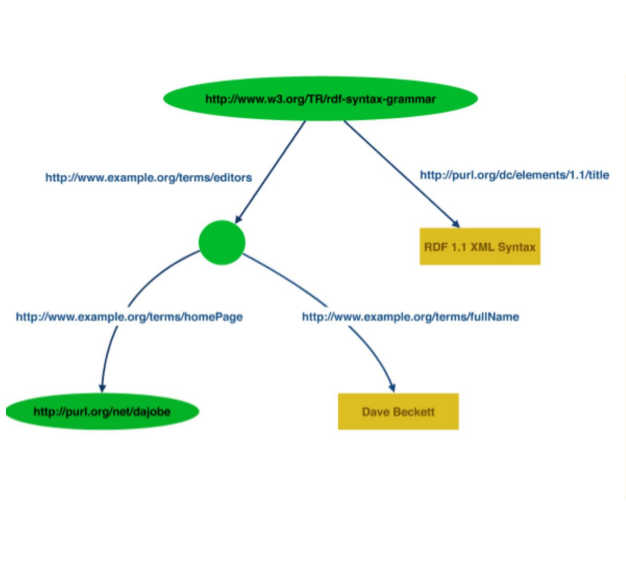
\includegraphics[width=0.5\textwidth]{_files/_images/rdf5.png}
    \caption{RDF abstract syntax}
    \label{fig:etichetta}
\end{figure}
\begin{figure}[h]
    \centering
    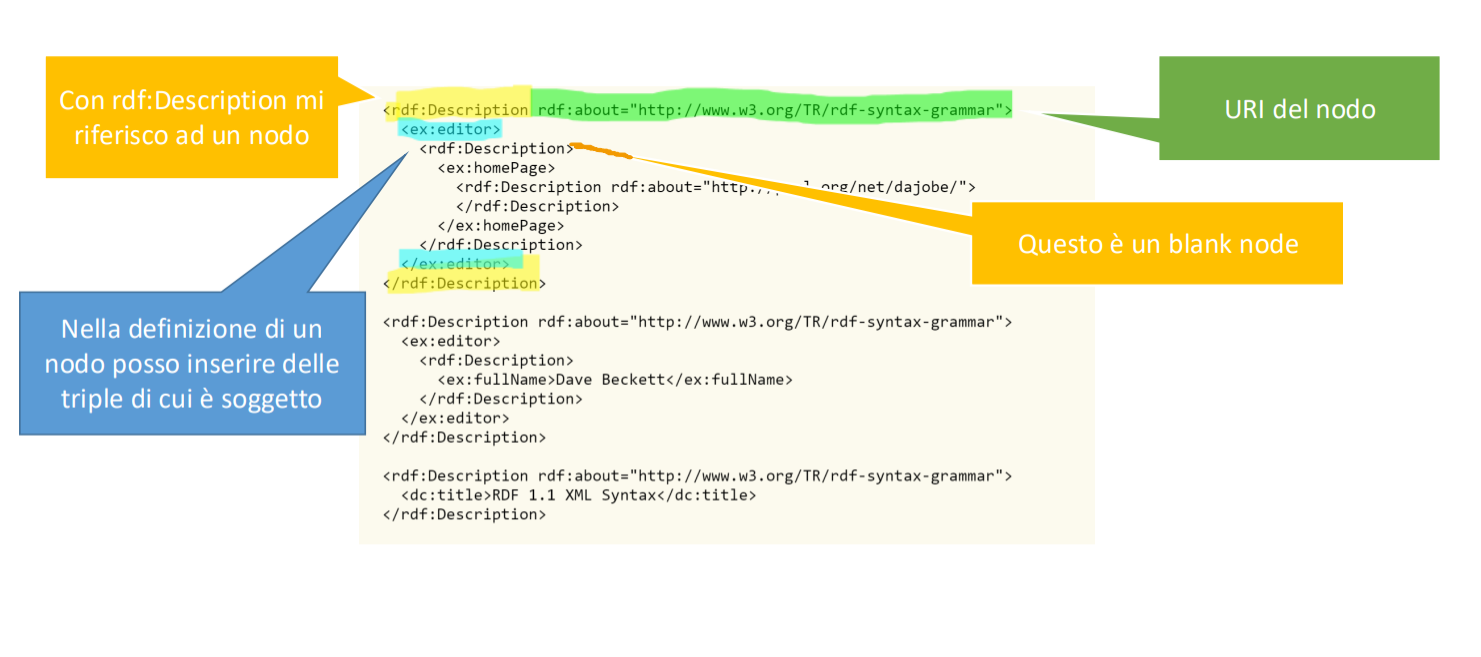
\includegraphics[width=1\textwidth]{_files/_images/rdf6.png}
    \caption{Implementazione nella serializzazione XML (Nota che i literal si rappresentano senza una particolare sintassi)}
    \label{fig:etichetta}
\end{figure}
\begin{figure}[h]
    \centering
    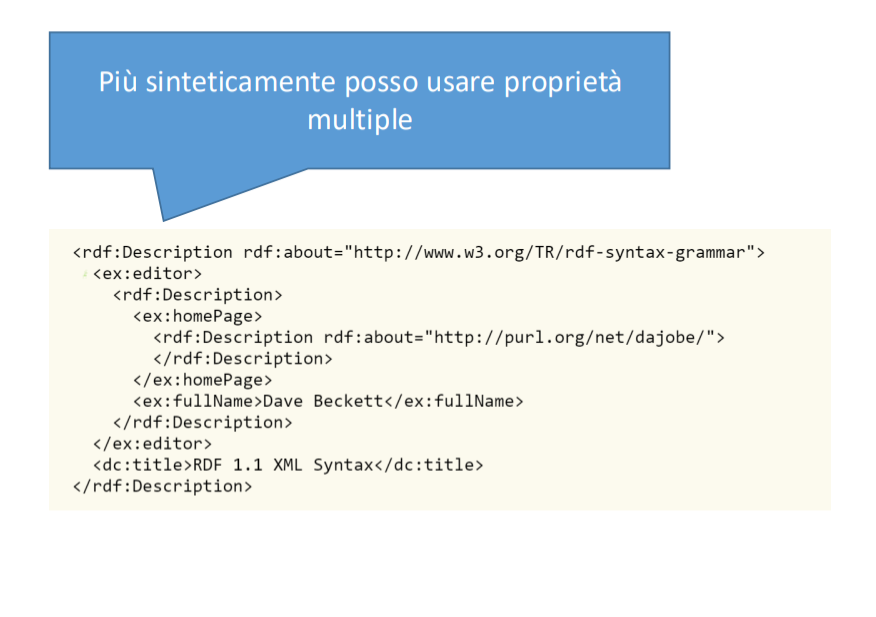
\includegraphics[width=0.6\textwidth]{_files/_images/rdf7.png}
    \caption{Posso immettere altre proprietà, come <dc:title> all'interno dello stesso nodo}
    \label{fig:etichetta}
\end{figure}

\begin{figure}[h]
    \centering
    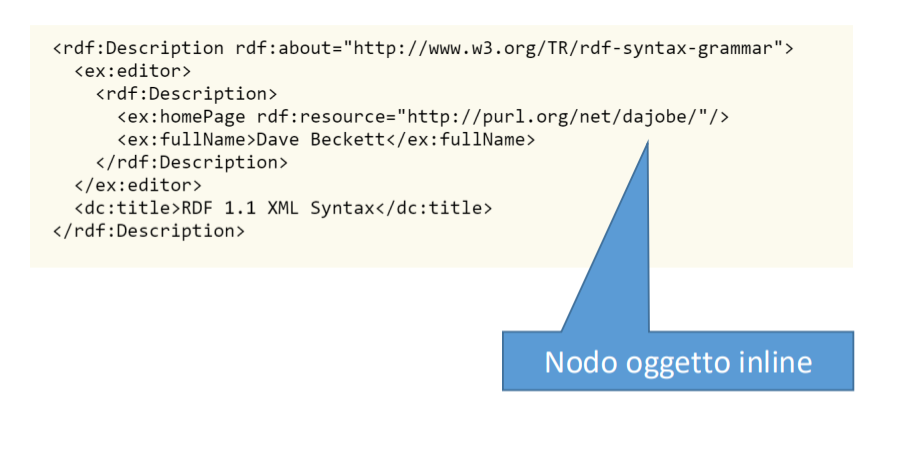
\includegraphics[width=0.6\textwidth]{_files/_images/rdf8.png}
    \caption{Si può usare rdf:resource, per specificare un nodo come oggetto inline}
    \label{fig:etichetta}
\end{figure}

\clearpage

\section{Vocabolari}
In RDF, per identificare risorse e proprietà si usano degli URI, come abbiamo visto in modo precedente.

\begin{definition}{Vocabolario RDF}
    Un vocabolario RDF è un insieme di termini identificati da URI, 
    generalmente classi e proprietà, utilizzati per descrivere le risorse di uno specifico dominio.Cioè un vocabolario,
    fornisce un insieme coerente di termini (classi e proprietà) per descrivere un certo dominio o ambito.
\end{definition}

\begin{example}{Esempio Vocabolario per http://example.org/university/}
    Un vocabolario per il dominio universitario definisce le classi e le proprietà necessarie a descrivere le risorse. Utilizzando la sintassi N-Triples/Turtle, un frammento del vocabolario è il seguente:
    
    \begin{lstlisting}[language=SQL, caption={Definizione del vocabolario universitario Turtle}]
@prefix ex: <http://example.org/university/> .
@prefix rdf: <http://www.w3.org/1999/02/22-rdf-syntax-ns#> .
@prefix rdfs: <http://www.w3.org/2000/01/rdf-schema#> .
@prefix foaf: <http://xmlns.com/foaf/0.1/> .

# Definizione delle Classi
ex:Student  a rdfs:Class ;
            rdfs:subClassOf foaf:Person .

ex:Course   a rdfs:Class .

# Definizione delle Proprieta
ex:teaches     a rdf:Property ;
               rdfs:domain ex:Professor ;
               rdfs:range  ex:Course .

ex:enrolledIn  a rdf:Property ;
               rdfs:domain ex:Student ;
               rdfs:range  ex:Course .
    \end{lstlisting}
    Come vedi in questo esempio, io sto andando a definire due tipi di classi e due tipi di proprietà, andando a creare il dizionario per "ex" (http://example.org/university/),
    gli altri dizionari invece, come rdf, e altri, già sono stati definiti, e li sto in un certo modo "importando".
    In questo esempio troviamo:
    \begin{itemize}
        \item \textbf{Classi} (\texttt{ex:Student}, \texttt{ex:Course}): identificano i concetti principali. Ad esempio, \texttt{Student} è definito come sottoclasse di \texttt{foaf:Person}.
        \item \textbf{Proprietà} (\texttt{ex:teaches}, \texttt{ex:enrolledIn}): definiscono le relazioni tra le classi, specificandone dominio (\textit{domain}) e codominio (\textit{range}).
    \end{itemize}
\end{example}

\begin{definition}{NameSpace}
    Il namespace è la parte comune di URI ai termini del vocabolario che stiamo definendo (nel caso di sopra http://example.org/university/ ).
    Quindi il namespace, è proprio l'URI di base, che si sceglie come parte comune per identificare e costruire in modo univoco gli URI completi di tutte le risorse, le classi e le proprietà di quel vocabolario, consentendo di abbreviarle tramite l'uso di un prefisso (QName) e un nome locale.
\end{definition}

I termini di un vocabolario possono essere rappresentati tramite QName, usando lo stesso prefisso per gli URI che condividono un namespace.
Ad esempio per il vocabolario di prima si potrebbe decidere si usare come prefisso "ex:", per "http://example.org/university/".


Quindi:
\begin{itemize}
    \item Si sceglie un unico namespace che raccoglie i termini del vocabolario, ovvero tutti gli URIref che condividono quel namespace come prefisso.
    \item  Se un namespace è deferenziabile allora la pagina web corrispondente fornisce informazioni
    sulla natura del vocabolario e il significato inteso dei suoi termini. Nota: questa è solo una buona
    pratica, RDF non assicura che un URI debba corrispondere ad un risorsa Web-retrivable
\end{itemize}

\begin{observation}{Stesso namespace}
   Un vocabolario non è obbligato tecnicamente ad avere tutti i suoi URI sotto lo stesso namespace, 
   ma normalmente è progettato così, perché rende il vocabolario più coerente e facilmente gestibile.
\end{observation}

\subsection{Un esempio di vocabolario : Foaf}
Il vocabolario FOAF (Friend of a Friend) definisce, tra gli altri:
\begin{itemize}
    \item \textbf{Classe} : foaf:Person
    \item \textbf{Proprietà} : foaf:name, foaf:knows, foaf:mbox,\dots
\end{itemize}
\subsection{Utilizzo di un Dizionario}
Una volta che ad esempio il W3C, ha definito il dizionario, quello che si può fare è "importare" il dizionario:
\begin{lstlisting}
@prefix rdf: <http://www.w3.org/1999/02/22-rdf-syntax-ns#> . // li puoi vedere come degli import
@prefix ex: <http://example.org/> .

ex:LaMiaPlaylist a rdf:Seq ;
    rdf:_1 ex:CanzoneA ;
    rdf:_2 ex:CanzoneB .
\end{lstlisting}

Quando poi si andrà a deferenziale : rdf:Seq, quello che succede è che si avrà l'URI : \url{http://www.w3.org/1999/02/22-rdf-syntax-ns#Seq} che sarà la risorsa descritta nel dizionario.


\section{Containers}
Il dizionario rdf, definisce alcuni tipi primitivi, detti container, per descrivere informazioni aggregate.
I container possono essere:
\begin{itemize}
    \item \textbf{Seq} : sequenza ordinata di nodi.
    \item \textbf{Bag} : collezione non ordinata di nodi.
    \item \textbf{Alt} :  lista di alternative equivalenti.
\end{itemize}
E' possibile avere ripetizioni, non vi è nessun meccanismo che forzi valori univoci.
RDF fornisce dei predicati built-in rdf:\_n per riferirsi ai vari componenti di container. Questi
predicati sono usati per istanziare indifferentemente Seq, Bag, o Alt ma chiaramente la
numerazione è significativa solo per le Seq.

\begin{figure}[htbp]
    \centering
    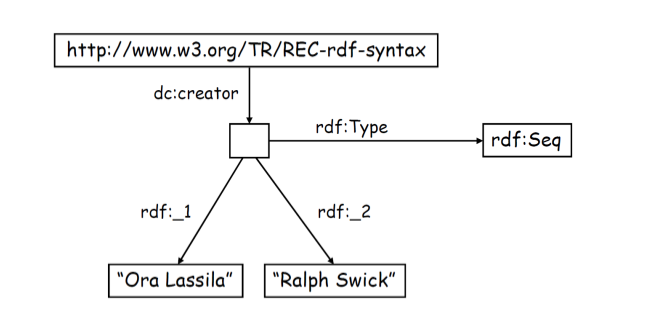
\includegraphics[width=0.7\textwidth]{_files/_images/rdf3.png}
    \caption{Esempio di Container}
    \label{fig:etichetta}
\end{figure}
\begin{lstlisting}
<http://www.w3.org/TR/REC-rdf-syntax> dc:creator _:seq.
_:seq rdf:Type rdf:Seq.
_:seq rdf:_1 "Ora Lassila".
_:seq rdf:_2 "Ralph Swick".
\end{lstlisting}
Qui tramite il dizionario rdf, stiamo definendo un container, dove gli elementi (in questo caso ordinati) sono quelle due stringhe.
\newpage

\section{Reificazione}
La reificazione è il meccanismo on cui in RDF è possibile prendere un'intera tripla (un statement) e trasformarla in una risorsa del grafo.
RDF fornisce dei predicati built-in per la reificazione:
\begin{itemize}
    \item \textbf{rdf:statement} : La classe che definisce che una determinata risorsa è una tripla reificata.   
    \item \textbf{rdf:subject} : Il predicato che indica qual è il soggetto della tripla originale.
    \item \textbf{rdf:predicate} : Il predicato che indica qual è il predicato della tripla originale.
    \item \textbf{rdf:object} : Il predicato che indica qual è l'oggetto della tripla originale.
\end{itemize}
\begin{figure}[htbp]
    \centering
    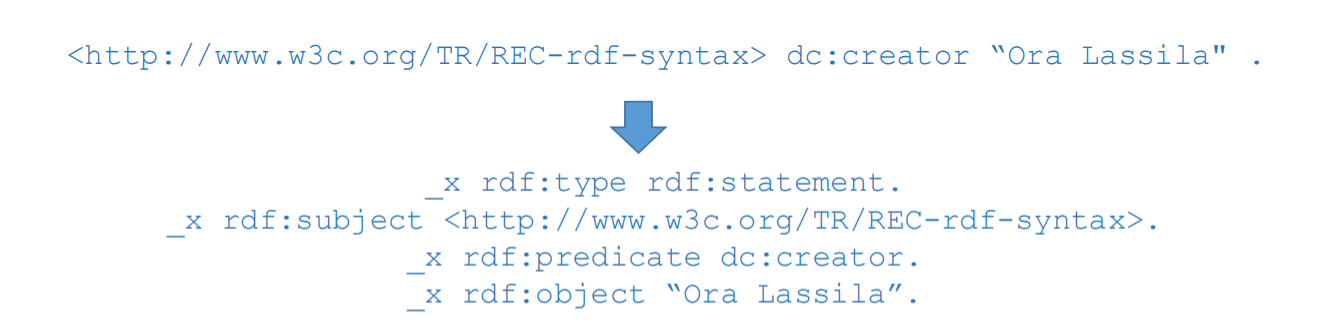
\includegraphics[width=0.7\textwidth]{_files/_images/rdf4.png}
    \caption{Esempio di reificazione dello statement}
    \label{fig:etichetta}
\end{figure}
\textbf{Ora lo statement è identificato dal blank node \_x}, ed è possibile esprimere il fatto che la Digital Library ha scritto questo statement
\begin{center}
    \_x dc:creator ``Digital Library''.
\end{center}


\section{RDFS}
RDFS è un vocabolario creato dal W3C, questo vocabolario introduce la capacità di creare gerarchie e vincoli di base.
\textbf{Si può vedere come un estensione del vocabolario base di RDF.}, che aggiunge una modellazione ad oggetti.
Nello specificio il vocabolario RDFS definisce un insieme di predicati che definiscono classi,domini,codomini e consentono di rappresentare il fatto che:
\begin{itemize}
    \item Un individuo appartiene ad una classe. (Tom è un gatto)
    \item Una classe è sottoclasse di un'altra classe. (i gatti sono felini)
    \item Il dominio e il codominio di una proprietà. (il dominio e il codominio di \texttt{friend\_of} è Person)
\end{itemize}

Il vocabolario RDFS, è disponibile in diverse serializzazioni (praticamente tutte quelle che abbiamo visto), noi useremo \textbf{la sintassi di Turtle}.

\subsection{Vocabolario per le classi}
Le classi permettono di raggruppare le risorse (i nodi del nostro grafo) in insiemi concettuali.

\begin{itemize}
    \item \textbf{rdfs:Class} (una risorsa e' una classe). \\
    Si utilizza per dichiarare l'esistenza di un concetto generale all'interno del dominio. Quando dichiariamo qualcosa come \texttt{rdfs:Class}, stiamo creando il ``contenitore'' concettuale.
    
    \item \textbf{rdf:type} (una risorsa e' un'istanza di una classe). \\
    \textit{[Nota: Appartiene al vocabolario RDF di base]}. Questo e' il predicato che collega un individuo specifico (una risorsa concreta) alla sua classe di appartenenza. Rappresenta la relazione ``is-a'' a livello di istanza (es. ``Mario e' un Uomo''), cioè
    definisce che una risorsa è un'istanza di una classe.
    
    \item \textbf{rdfs:subClassOf} (una classe e' sottoclasse di un'altra). \\
    Permette di creare tassonomie e gerarchie. Se la classe A e' sottoclasse di B, ogni \textbf{istanza di A e' implicitamente anche un'istanza di B}.
\end{itemize}

\paragraph{Esempio Pratico (Classi):}
Immaginiamo di voler modellare il concetto di essere umano e di studente.

\begin{verbatim}
# Definiamo due classi
ex:Persona rdf:type rdfs:Class .
ex:Studente rdf:type rdfs:Class .

# Creiamo la gerarchia: ogni Studente e' una Persona
ex:Studente rdfs:subClassOf ex:Persona .

# Creiamo un'istanza (un dato concreto)
ex:Mario Rossi rdf:type ex:Studente .
\end{verbatim}

\noindent
\textit{Inferenza logica:} Grazie a \texttt{rdfs:subClassOf}, un motore di inferenza che legge questo grafo dedurra' automaticamente la tripla implicita \texttt{ex:Mario Rossi rdf:type ex:Persona}, anche se noi non l'abbiamo scritta esplicitamente.
Questo perchè grazie a \textbf{rdf:type}, posso dire che Mario Rossi è un'istanza di Studente, ma grazie a \textbf{rdfs:subClassOf}, posso dire che 
ogni istanza di studente è anche \textbf{un'istanza} di una persona, quindi Mario rossi è un'istanza di Persona, e questo si esprime nel seguente modo:
ex:Mario Rossi rdf:type ex:Persona . Questo perchè con rdf:type si esprime "è un'istanza".



\subsection{Vocabolario per le proprieta'}
Le proprieta' definiscono i tipi di archi che collegano i nodi nel grafo, descrivendo le relazioni tra le risorse.

\begin{itemize}
    \item \textbf{rdf:Property} (una risorsa e' una proprieta'). \\
    \textit{[Nota: Appartiene al vocabolario RDF]}. Serve a dichiarare che un certo termine puo' essere usato come predicato in una tripla.
    
    \item \textbf{rdfs:subPropertyOf} (una proprieta' e' sottoproprieta' di un'altra). \\
    Crea una gerarchia tra le relazioni stesse. Se la proprieta' P1 e' sottoproprieta' di P2, ogni volta che due nodi sono collegati da P1, il sistema deduce che sono collegati anche da P2.
    
    \item \textbf{rdfs:domain} (il dominio). \\
    Vincola il Soggetto della tripla. Se una proprieta' ha come dominio la classe C, significa che qualsiasi risorsa che usi questa proprieta' come soggetto appartiene implicitamente alla classe C.
    
    \item \textbf{rdfs:range} (il codominio o range). \\
    Vincola l'Oggetto della tripla. Se una proprieta' ha come range la classe C, il valore di arrivo della relazione sara' implicitamente un'istanza della classe C.
\end{itemize}

\paragraph{Esempio Pratico (Proprieta'):}
Definiamo una relazione generale di conoscenza e una piu' specifica di amicizia, applicando dei vincoli.

\begin{verbatim}
# Definiamo la proprieta' generale "conosce"
ex:conosce rdf:type rdf:Property ;
           rdfs:domain ex:Persona ;
           rdfs:range ex:Persona .

# Definiamo la proprieta' piu' specifica "amico di"
ex:amicoDi rdf:type rdf:Property ;
           rdfs:subPropertyOf ex:conosce .

# Dati concreti nel grafo
ex:Mario Rossi ex:amicoDi ex:Luigi Bianchi .
\end{verbatim}

\noindent
\textit{Inferenze logiche generate in questo esempio:}
\begin{enumerate}
    \item Poiche' \texttt{amicoDi} e' sottoproprieta' di \texttt{conosce}, il sistema deduce: \\ \texttt{ex:Mario Rossi ex:conosce ex:Luigi Bianchi}.
    \item Poiche' chiunque usi il predicato \texttt{conosce} deve appartenere alla classe \texttt{Persona} (vincolo di dominio), il sistema deduce che Mario Rossi e' una Persona.
    \item Poiche' il target del predicato \texttt{conosce} deve essere della classe \texttt{Persona} (vincolo di range), il sistema deduce che anche Luigi Bianchi e' una Persona.
\end{enumerate}

Un esempio di pezzo del dizionario (serializzato in Turtle):
\begin{lstlisting}
@prefix rdf: <http://www.w3.org/1999/02/22-rdf-syntax-ns#> .
@prefix rdfs: <http://www.w3.org/2000/01/rdf-schema#> .

rdfs:Class rdf:type rdfs:Class ;
           rdfs:subClassOf rdfs:Resource ;
           rdfs:label "Class" ;
           rdfs:comment "The class of classes." .
\end{lstlisting}
\subsection{Tassonomie}
Una tassonomia è una gerarchia di classi, dalle più specifiche alle più generali.
\begin{figure}[htbp]
    \centering
    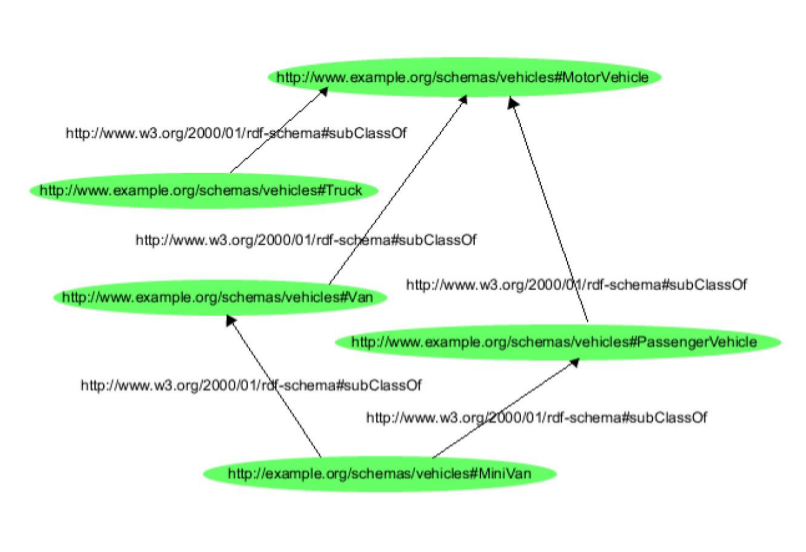
\includegraphics[width=0.7\textwidth]{_files/_images/rdf9.png}
    \caption{Esempio di Tassonomia, cioè di gerarchia fra classi, questa può essere rappresentata in Turtle o diverse serializzazioni.}
    \label{fig:etichetta}
\end{figure}

\clearpage

\begin{figure}[h]
    \centering
    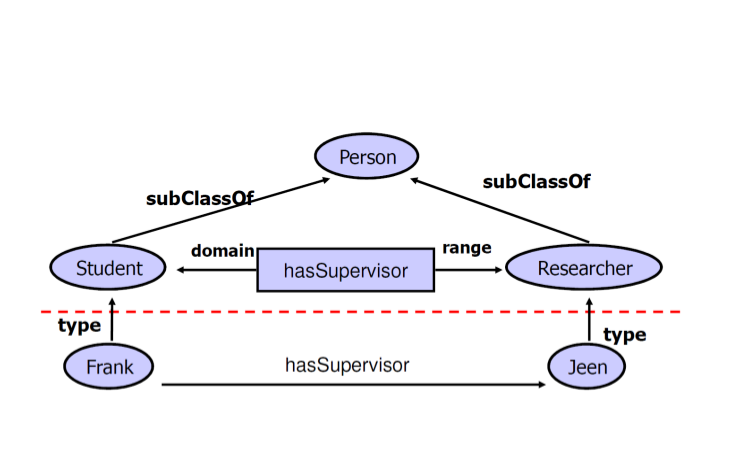
\includegraphics[width=0.7\textwidth]{_files/_images/rdf10.png}
    \caption{Grafo delle informazioni esplicite.}
    \label{fig:etichetta}
\end{figure}
Da questo grafo posso infierire due cose:
\begin{itemize}
    \item (Frank rdf:type Person)
    \item (Jeen rdf:type Person)
\end{itemize}



\subsection{Differenza Fra Vocabolario e Ontologia}

Nel contesto del Web Semantico, i concetti di \textit{vocabolario} e
\textit{ontologia} sono strettamente correlati, ma non completamente
sovrapponibili.

Un \textbf{vocabolario} definisce principalmente un insieme di termini
utilizzabili per descrivere un determinato dominio. Tali termini possono
essere rappresentati, ad esempio, attraverso classi e proprietà RDF. Per
esempio, un vocabolario potrebbe definire la classe \texttt{Person} e la
proprietà \texttt{knows}:

\begin{verbatim}
:Person a rdfs:Class .
:knows a rdf:Property .
\end{verbatim}

In questo caso, il vocabolario introduce i concetti e le proprietà che
possono essere utilizzati nella descrizione delle risorse, senza
necessariamente specificare una conoscenza complessa sulle relazioni
esistenti tra tali concetti.

Un'\textbf{ontologia}, invece, estende questo concetto introducendo una
descrizione formale della semantica del dominio. Oltre a definire classi e
proprietà, un'ontologia può specificare relazioni tra classi, gerarchie,
vincoli e assiomi che descrivono come i diversi concetti sono collegati tra
loro.

Ad esempio, è possibile stabilire che \texttt{Student} sia una
sottoclasse di \texttt{Person}:

\begin{verbatim}
:Student rdfs:subClassOf :Person .
\end{verbatim}

Oppure, utilizzando OWL, è possibile esprimere vincoli più complessi.
Ad esempio:

\[
\mathit{Student} \sqsubseteq
\exists\,\mathit{attends}.\mathit{University}
\]

indica che ogni individuo appartenente alla classe \texttt{Student} deve
essere collegato, tramite la proprietà \texttt{attends}, ad almeno un
individuo appartenente alla classe \texttt{University}.

La differenza può quindi essere riassunta nel seguente modo:

\begin{itemize}
    \item il \textbf{vocabolario} definisce i termini, le classi e le
    proprietà utilizzabili per descrivere un dominio;
    \item l'\textbf{ontologia} aggiunge a tali termini una semantica
    formale, definendo relazioni, gerarchie, vincoli e assiomi che
    descrivono il dominio e che possono essere utilizzati per effettuare
    inferenze.
\end{itemize}

È importante sottolineare che la distinzione non è sempre netta: un
vocabolario sufficientemente ricco può contenere anche informazioni
semantiche e, in senso lato, essere considerato un'ontologia. Per questo
motivo, nella letteratura sul Web Semantico i due termini vengono talvolta
utilizzati in modo intercambiabile. La distinzione precedente è quindi
soprattutto utile per comprendere il diverso livello di formalizzazione
della conoscenza rappresentata.


\newpage
\section{SPARQL}
SPARQL (Simple Protocol and RDF Query Language) è il linguaggio di query per interrogare modelli RDF.
Permette di cercare informazioni dentro un grafo RDF specificando pattern di triple da
trovare.
\begin{warning}{SPARQL è indipendente dalla serializzazione}
    SPARQL interroga il grafo RDF, \textbf{tramite una sintassi simile a Turtle}, \textbf{ma questo non implica che può interrogare solo dati in Turtle},
    anzi, quello che fa SPARQL è interrogare il grafo RDF, che viene rappresentato da tutte le serializzazioni.

    
    \textbf{Quindi SPARQL è indipendente dalla serializzazione dei dati}
\end{warning}

\begin{lstlisting}[caption={Query SPARQL per capitali e paesi nel continente africano}]
PREFIX abc: <http://mynamespace.com/exampleOntology#>
SELECT ?capital ?country
WHERE { ?x abc:cityname ?capital.
        ?y abc:countryname ?country.
        ?x abc:isCapitalOf ?y.
        ?y abc:isInContinent abc:africa. }
\end{lstlisting}

In pratica, una query SPARQL descrive la forma delle triple che vogliamo trovare.
\begin{itemize}
    \item \textbf{Le variabili} : sono identificate dal prefisso ? , ad esempio ?person,?label
    \item La clausola \textbf{WHERE} contiene le condizioni della query sotto forma di triple, cioè soggetto,
predicato e oggetto, questa restituisce una \textbf{tabella di binding delle variabili.}
    \item La clausola \textbf{SELECT} specifica invece quali variabili devono essere restituite nel risultato
finale
\end{itemize}
La struttura base è quindi:
\begin{lstlisting}[caption={Struttura base di una query SPARQL}]
SELECT ?variabile
WHERE {
?soggetto ?predicato ?oggetto .
}
\end{lstlisting}
Qui ?soggetto , ?predicato e ?oggetto sono variabili. Il motore SPARQL proverà a sostituirle con valori reali presenti nel grafo RDF.
\subsection{Esempi pratici di interrogazioni}
Per ottenere una lista di tutte le risorse che hanno un'etichetta, cioè una label, si può scrivere:
\begin{lstlisting}
PREFIX rdfs: <http://www.w3.org/2000/01/rdf-schema#>
SELECT ?resource ?label
WHERE {
?resource rdfs:label ?label .
} 
\end{lstlisting}
Supponiamo di avere il grafo definito da questo codice:
\begin{lstlisting}
ex:Dante ex:HaScritto ex:DivinaCommedia .
ex:Dante ex:HaScritto ex:VitaNova .
ex:Petrarca ex:HaScritto ex:Canzoniere .
\end{lstlisting}
e la query è:
\begin{lstlisting}
SELECT ?persona ?opera
WHERE {
?persona ex:HaScritto ?opera .
}
\end{lstlisting}
Quello che succede è che nel where viene costruita una tabella di binding (come abbiamo detto prima), in questo caso le
colonne saranno fatto in questo modo:

\begin{center}
\begin{tabular}{|l|l|}
\hline
\textbf{?persona} & \textbf{?opera} \\ \hline
ex:Dante & ex:VitaNova \\ \hline
ex:Petrarca & ex:Canzoniere \\ \hline
ex:Dante & ex:DivinaCommedia \\ \hline
\end{tabular}
\end{center}
La select poi da questa tabella, seleziona solo ?persona ed ?opera che già ci sono.


\begin{definition}{Basic Graph Pattern}
Un BGP è un insieme di triple pattern, \textbf{cioè triple RDF in cui alcuni elementi possono essere variabili (giustamente perchè siamo in SPARQL).}
\end{definition}
\begin{example}{Esempio di Basic Graph Pattern}
Supponiamo di avere la query:
\begin{lstlisting}
SELECT ?person
WHERE {
    ?person :worksFor :Google .
}
\end{lstlisting}
Un esempio di BGP è :
\begin{center}
    ?person :worksFor :Google .
\end{center}
Il concetto fondamentale è che un BGP, può contenere piu triple di pattern.
Per esempio:
\begin{lstlisting}
SELECT ?person ?company
WHERE {
    ?person :worksFor ?company .
    ?person :knows :Luigi .
}
\end{lstlisting}
Il BGP è formato da due triple di pattern:
\begin{center}
?person :worksFor ?company . \\
?person :knows    :Luigi    .
\end{center}
\end{example}
\begin{definition}{Group Graph Pattern}
Un insieme di pattern SPARQL raggruppati tra \{\}, che può contenere anche BGP, OPTIONAL, UNION, FILTER, ecc, quindi un contenitore per altri pattern.
\end{definition}
\begin{example}{Esempio di GGP}
Un GGP è piu generale di un BGP, un GGP è \textbf{tutto quello che vi è dentro le parentesi graffe}.
\begin{lstlisting}
{
    ?person :worksFor ?company .

    OPTIONAL {
        ?person :knows ?friend .
    }
}
\end{lstlisting}
\begin{center}
\begin{forest}
  for tree={
    font=\ttfamily,
    grow'=0,
    child anchor=west,
    parent anchor=south,
    anchor=west,
    calign=child,
    edge path={
      \noexpand\path [\forestoption{edge}]
      (!u.south west) +(7.5pt,0) |- (.child anchor)\forestoption{edge label};
    },
    before typesetting nodes={
      if n=1 {
        insert before={[,phantom]}
      }{}
    },
    fit=band,
    s sep=20pt,
    l sep=15pt
  }
[GGP
  [BGP
    [?person :worksFor ?company]
  ]
  [OPTIONAL
    [GGP
      [BGP
        [?person :knows ?friend]
      ]
    ]
  ]
]
\end{forest}
\end{center}
\end{example}
\subsection{Solution Mapping}
Il concetto di Solution Mapping, indicato spesso con $\mu$, serve a rappresentare formalmente
una singola soluzione di una query SPARQL. Un solution mapping rappresenta una riga della tabella fuoriuscente dal WHERE.


Un solution mapping, associa alle variabili della query a termini RDF. Formalmente un Solution Mapping è una funzione, che è definita:
\begin{center}
    $\mu$ : Var $\to$ RDFTerm
\end{center}
dove
\begin{itemize}
    \item \textbf{Var} : sono le variabili della query, ad esempio nel where, se ho da riempire ?person e ?film, allora il dominio sarà quello
    \item \textbf{RDFTerm} :  possono essere URI, letterali o blank node.
\end{itemize}

Per esempio, se una query contiene ?film e ?person , una possibile funzione è:
\begin{itemize}
    \item $\mu(?film)$ = eg:Arrival
    \item $\mu(?person)$ = eg:Adams
\end{itemize}
In pratica, $\mu$ corrisponde ad una riga del risultato, ovviamente la tabella fuoriuscente non sarà solo una riga del risultato,
ma sarà un multiset, cioè
\[
\{\mu_1, \mu_2, \dots\}
\]
\subsection{Blank Node nei risultati della query}

Una tabella di risultati SPARQL può contenere anche \textbf{blank node}.

È importante ricordare che gli identificatori associati ai blank node sono \textbf{locali al grafo RDF in cui vengono utilizzati}: non sono URI e non costituiscono identificatori globali della risorsa.

Ad esempio, in un grafo RDF possiamo avere:

\begin{lstlisting}
:Mario :hasAddress _:b1 .
_:b1 :city "Napoli" .
\end{lstlisting}

In questo caso, \texttt{\_:b1} identifica un blank node \textbf{all'interno del contesto del grafo}. Non significa che esista una risorsa globalmente identificata dall'identificatore \texttt{\_:b1}.

Di conseguenza, quando un blank node viene restituito come risultato di una query SPARQL, \textbf{l'identificatore utilizzato nella tabella dei risultati non deve necessariamente coincidere con quello utilizzato nel grafo originale}.

Ad esempio, consideriamo la query:

\begin{lstlisting}
SELECT ?address
WHERE {
:Mario :hasAddress ?address .
}
\end{lstlisting}

Se nel grafo abbiamo:

\begin{lstlisting}
:Mario :hasAddress _:b1 .
_:b1 :city "Napoli" .
\end{lstlisting}

il risultato potrebbe essere rappresentato come:

\begin{center}
\begin{tabular}{|c|}
\hline
\textbf{?address} \\ \hline
\texttt{\_:b0} \\ \hline
\end{tabular}
\end{center}

Qui \texttt{\_:b0} rappresenta il blank node restituito come valore di \texttt{?address}, ma \textbf{non deve essere interpretato come un nuovo identificatore globale} e non è necessario che coincida con \texttt{\_:b1}, utilizzato nel grafo originale.

In altre parole:

\begin{itemize}
\item nel grafo originale il blank node può essere rappresentato come \texttt{\_:b1};
\item nei risultati della query lo stesso blank node può essere rappresentato come \texttt{\_:b0};
\item ciò che conta è che il blank node sia correttamente identificato \textbf{all'interno del contesto in cui viene rappresentato}, non il valore testuale dell'etichetta.
\end{itemize}

Pertanto, gli identificatori dei blank node sono \textbf{locali al contesto RDF} e non possono essere utilizzati come identificatori globali per riferirsi a una risorsa al di fuori di tale contesto.

\subsection{Utilizzo di Select}
La forma di query \texttt{SELECT} è la più utilizzata in SPARQL. Il suo scopo è quello di estrarre e restituire i valori legati a specifiche variabili definite nella clausola \texttt{WHERE}. Il risultato di una query \texttt{SELECT} è un insieme di solution mapping in cui le colonne corrispondono alle variabili richieste e le righe rappresentano ogni singola combinazione di valori (soluzione) trovata all'interno del grafo.

È il costrutto ideale quando si desidera estrapolare informazioni testuali o elenchi da mostrare a un utente o far elaborare a un'applicazione.

\textbf{Esempio Pratico:}
Supponiamo di voler trovare il nome e l'indirizzo email di tutte le persone presenti nel nostro database utilizzando il vocabolario FOAF (\textit{Friend of a Friend}).

\begin{lstlisting}
PREFIX foaf: <http://xmlns.com/foaf/0.1/>

SELECT ?nome ?email
WHERE {
  ?persona a foaf:Person ;
           foaf:name ?nome ;
           foaf:mbox ?email .
}
\end{lstlisting}
In questo caso, il motore SPARQL restituirà una tabella con due colonne (\texttt{?nome} e \texttt{?email}) contenenti rispettivamente i nomi e le caselle di posta elettronica trovati.

\subsection{Utilizzo di ASK}
La forma di query \texttt{ASK} serve per effettuare una verifica dell'esistenza di un determinato pattern. A differenza di \texttt{SELECT}, non restituisce i dati effettivi (non estrae stringhe, URI o numeri), ma si limita a rispondere con un valore booleano: \texttt{True} (Vero) se esiste almeno una soluzione nel dataset che soddisfa le condizioni della clausola \texttt{WHERE}, oppure \texttt{False} (Falso) in caso contrario.

Questo costrutto è estremamente utile ed efficiente per effettuare controlli rapidi. Poiché il database può fermare la ricerca al primo risultato trovato senza dover costruire una tabella completa, le query \texttt{ASK} sono generalmente molto più leggere.

\textbf{Esempio Pratico:}
Vogliamo semplicemente sapere se all'interno del database è presente una persona che si chiama "Mario Rossi".

\begin{lstlisting}
PREFIX foaf: <http://xmlns.com/foaf/0.1/>

ASK
WHERE {
  ?persona a foaf:Person ;
           foaf:name "Mario Rossi" .
}
\end{lstlisting}
Il risultato di questa query sarà il valore \texttt{true} se Mario Rossi esiste nel grafo, altrimenti \texttt{false}.

In generale il valore di ask sarà \texttt{true}, se esiste almeno una tripla nel Solution Mapping fuoriuscente, altrimenti \texttt{false}

\subsection{Utilizzo di Construct}
La forma \texttt{CONSTRUCT} è un potente strumento di manipolazione dei dati. Invece di restituire una tabella di risultati (come fa la \texttt{SELECT}), la \texttt{CONSTRUCT} restituisce un \textbf{nuovo grafo RDF}. 

Il funzionamento prevede di definire un "template" di triple subito dopo la parola chiave \texttt{CONSTRUCT}.

Per ogni soluzione trovata nella clausola \texttt{WHERE},\textbf{ i valori delle variabili vengono iniettati nel template scritto in CONSTRUCT per generare nuove triple RDF}. 

\textbf{Esempio Pratico:}
Immaginiamo di avere un database in cui le persone sono definite tramite il vocabolario FOAF. Vogliamo estrarre questi dati e generare un nuovo grafo RDF in cui le stesse persone sono espresse usando il vocabolario \texttt{vCard}.

\begin{lstlisting}
PREFIX foaf: <http://xmlns.com/foaf/0.1/>
PREFIX vcard: <http://www.w3.org/2001/vcard-rdf/3.0#>

CONSTRUCT {
  # Template del nuovo grafo
  ?persona a vcard:Individual ;
           vcard:FN ?nome .
}
WHERE {
  # Ricerca nel grafo originale
  ?persona a foaf:Person ;
           foaf:name ?nome .
}
\end{lstlisting}
L'output di questa query non sarà una tabella di nomi, ma un vero e proprio grafo RDF contenente le nuove triple tradotte.

\subsection{Utilizzo di Order By}
Per ordinare i risultati di una tabella, si può usare il costrutto \textbf{Order By}
\begin{lstlisting}
SELECT ?person (COUNT(*) AS ?friendCount)
WHERE {
?person <http://example.org/hasFriend> ?friend .
}
GROUP BY ?person
ORDER BY DESC(?friendCount)
LIMIT 1
\end{lstlisting}

\subsection{Utilizzo di OFFSET e LIMIT}
\textbf{OFFSET n} indica al motore SPARQL, di saltare i primi n risultati.
\begin{lstlisting}
ORDER BY DESC(?pop)
OFFSET 5
\end{lstlisting}
Salta i primi 5 risultati della tabella.


Spesso usato insieme a LIMIT, in questo modo:
\begin{lstlisting}
ORDER BY DESC(?pop)
OFFSET 5
LIMIT 10
\end{lstlisting}
Questa query ordina i risultati in base alla popolazione decrescente, salta i primi 5 risultati e poi
restituisce i successivi 10.

\subsection{La clausola Group By}
La clausola Group By viene usata per raggrupare un insieme di triple, per un dato valore.


Supponiamo che dal \textbf{where} ci escono questi dati:
\begin{table}[h]
\centering
\ttfamily
\begin{tabular}{ll}
?city & ?population \\
\hline
Roma & 2800000 \\
Roma & 100000 \\
Milano & 1400000 \\
Milano & 50000 \\
Napoli & 900000 \\
\end{tabular}
\end{table}


Se faccio:
\begin{lstlisting}
SELECT ?city (SUM(?population) AS ?total)
WHERE {
...
}
GROUP BY ?city
\end{lstlisting}

SPARQL crea i \textbf{gruppi(vengono chiamati proprio cosi)} (grazie a group by):
\begin{lstlisting}
Roma --> {2800000, 100000}
Milano --> {1400000, 50000}
Napoli --> {900000}
\end{lstlisting}
e poi applica da qui posso applicare la Funzioni principali di aggregazione separatamente a
ogni gruppo, ad esempio SUM :
\begin{lstlisting}
Roma   --> 2900000
Milano  --> 1450000
Napoli  --> 900000
\end{lstlisting}
Queste funzioni principali di aggregazione, spesso si utilizzano insieme a Group By, perchè
usarle da sole è poco utile molte volte.    

\subsubsection{Funzioni principali di aggregazione}
\textbf{Operatore COUNT}


L'operatore \texttt{COUNT} è una funzione di aggregazione che calcola il numero totale di soluzioni, righe o valori associati a una specifica variabile all'interno di un insieme di risultati.

In SPARQL, l'uso delle funzioni di aggregazione richiede spesso la clausola \texttt{GROUP BY} per raggruppare i dati secondo una o più variabili.

Proprietà fondamentali di \texttt{COUNT}:
\begin{itemize}
    \item \textbf{\texttt{COUNT(*)}:} Conta il numero totale di righe/soluzioni nel gruppo, incluse quelle con valori non definiti (\textit{unbound}).
    \item \textbf{\texttt{COUNT(?var)}:} Conta solo il numero di soluzioni in cui la variabile \texttt{?var} è definita (\textit{bound}).
    \item \textbf{\texttt{COUNT(DISTINCT ?var)}:} Conta solo i valori unici e distinti assunti dalla variabile \texttt{?var}, eliminando i duplicati.
\end{itemize}

\textbf{Esempio 1: Conteggio totale per gruppo}

Supponiamo di voler contare quanti prodotti appartengono a ciascuna categoria:

\begin{verbatim}
SELECT ?categoria (COUNT(?prodotto) AS ?numeroProdotti)
WHERE {
    ?prodotto :appartieneA ?categoria .
}
GROUP BY ?categoria
\end{verbatim}

\paragraph{Esempio con più colonne}

Anche quando una soluzione è composta da \textbf{più colonne}, \texttt{COUNT(*)} conta comunque il \textbf{numero di righe (soluzioni) appartenenti a ciascun gruppo}.

Ad esempio, supponiamo di avere la seguente tabella di risultati:

\begin{center}
\begin{tabular}{c|c|c}
\textbf{persona} & \textbf{amico} & \textbf{città} \\
\hline
Giuliano & Marco & Napoli \\
Giuliano & Luca & Roma \\
Giuliano & Anna & Napoli \\
Mario & Paolo & Napoli \\
Mario & Luca & Roma
\end{tabular}
\end{center}

Se utilizziamo:

\begin{verbatim}
SELECT ?persona (COUNT(*) AS ?numero)
WHERE {
?persona foaf:knows ?amico .
?amico :viveA ?citta .
}
GROUP BY ?persona
\end{verbatim}

Il risultato sarà:

\begin{center}
\begin{tabular}{c|c}
\textbf{persona} & \textbf{numero} \\
\hline
Giuliano & 3 \\
Mario & 2
\end{tabular}
\end{center}

Infatti, il gruppo di \texttt{Giuliano} contiene \textbf{3 righe}, mentre il gruppo di \texttt{Mario} contiene \textbf{2 righe}. Quindi \texttt{COUNT(*)} conta le \textbf{righe del gruppo}, indipendentemente dal numero di colonne presenti in ogni riga.

Se invece utilizziamo:

\begin{verbatim}
GROUP BY ?persona ?citta
\end{verbatim}

le righe vengono raggruppate considerando \textbf{sia la persona sia la città}:

\begin{center}
\begin{tabular}{c|c|c}
\textbf{persona} & \textbf{città} & \textbf{numero} \\
\hline
Giuliano & Napoli & 2 \\
Giuliano & Roma & 1 \\
Mario & Napoli & 1 \\
Mario & Roma & 1
\end{tabular}
\end{center}

In questo caso, ogni gruppo è determinato dalla coppia \texttt{(?persona, ?citta)} e \texttt{COUNT(*)} conta quante righe appartengono a ciascuna coppia.



\textbf{SUM} somma i valori numerici.
\begin{lstlisting}
(SUM(?population) AS ?totalPopulation)
\end{lstlisting}


\textbf{AVG}  calcola la media.
\begin{lstlisting}
(AVG(?population) AS ?avgPopulation)
\end{lstlisting}


\textbf{MIN} restituisce il minimo.
\begin{lstlisting}
(MIN(?age) AS ?minAge)
\end{lstlisting}


\textbf{MAX} restituisce il massimo.
\begin{lstlisting}
(MAX(?age) AS ?maxAge)
\end{lstlisting}

\subsection{La clausola HAVING}
La clausola HAVING viene utilizzata quando vogliamo applicare una condizione ai risultati che
abbiamo raggrupato.


Supponiamo di voler visualizzare solo i lavori che hanno più di 100 persone associate.
\begin{lstlisting}
SELECT ?job (COUNT(?person) AS ?numPeople)
WHERE {
?person eg:hasJob ?job .
}
GROUP BY ?job
HAVING (COUNT(?person) > 100)
\end{lstlisting}
\textbf{Nota che io qui non posso usare ?numPeople, perchè quello è il nome che si assegna alla colonna}
\textbf{HAVING si usa sui gruppi dopo GROUP BY}

\subsection{FILTER}
FILTER agisce dopo il matching: prima si trovano tutte le soluzioni che soddisfano i triple
pattern, poi si scartano quelle per cui l'espressione del filtro valuta a false.

FILTER agisce in modo tale che, vengono prima trovate tutte le triple che fanno
MATCHING, e poi viene applicata la condizione.

\begin{lstlisting}
SELECT ?child1 ?child2
WHERE {
?parent <http://example.org/hasChild> ?child1, ?child2 .
FILTER (?child1 != ?child2)
}
\end{lstlisting}

Viene prima riempita la tabella dei Solution Mapping, poi successivamente, vengono eliminate alcune righe, con il costrutto FILTER.


Ci sono due regole importante delle triple.
\begin{itemize}
    \item \textbf{i filtri non creano nuovi mapping}, cioè non posso usare una nuova variabile, se scrivo FILTER(?age > 18), la variabile ?age, deve comparire, da qualche parte nel WHERE.
    \item \textbf{ l’ordine del filtro è irrilevante},quindi posso mettere dove voglio il FILTER all'interno del WHERE.
\end{itemize}

\subsection{La clausola OPTIONAL}
\textbf{OPTIONAL permette di aggiungere informazioni opzionali a una soluzione.}


Il pattern generale è questo:
\begin{lstlisting}
WHERE {
    Pattern1 .
    OPTIONAL {
        Pattern2 .
    }
}
\end{lstlisting}
\textbf{Prima si cercano le soluzioni che soddisfano i pattern obbligatori,per ciascuna soluzione trovata si prova a verificare il pattern dentro optional}
Se il pattern trova corrispondenza, viene aggiunta il valore della colonna della tabella corrispondente al solution mapping, se non trova corrispondenza, allora 
viene aggiunto il valore \textbf{unbound}


\paragraph{Esempio}
Supponiamo di avere il seguente grafo:
\begin{lstlisting}
:Giuliano foaf:name "Giuliano" .
:Giuliano foaf:age 22 .
:Marco foaf:name "Marco" .
\end{lstlisting}

Supponiamo di avere la seguente query:
\begin{lstlisting}
    WHERE {
    ?persona foaf:name ?nome .

    OPTIONAL {
        ?persona foaf:age ?eta .
    }
}
\end{lstlisting}
Allora il pipeline dell'esecuzione è:
\begin{itemize}
    \item Prima ottieni \textbf{dal pattern obbligatorio}:
    \begin{lstlisting}
        Giuliano --> "Giuliano"
        Marco    --> "Marco"
    \end{lstlisting}
    \item Poi il motore prova l'OPTIONAL, per ogni riga:
    \begin{lstlisting}
        Giuliano --> ha age --> 22
        Marco    --> non ha age --> unbound
    \end{lstlisting}
\end{itemize}
Il risultato finale è:
\begin{table}[h]
\centering
\begin{tabular}{|l|l||l|}
\hline
\textbf{?persona} & \textbf{?nome} & \textbf{?eta} \\ \hline
:Giuliano          & Giuliano & 22      \\ \hline
:Marco             & Marco    & UNBOUND \\ \hline
\end{tabular}
\end{table}


Supponiamo ora di avere la seguente query:
\begin{lstlisting}
SELECT ?person ?age
WHERE {
    OPTIONAL {
        ?person foaf:age ?age .
    }
}
\end{lstlisting}
Qui non c'è un pattern obbligatorio, OPTIONAL,si comporta esattamente come il pattern all'interno,quindi il solution mapping trovato è:
\begin{table}[h]
\centering
\begin{tabular}{|l|l|}
\hline
\textbf{?person} & \textbf{?age} \\ \hline
:Giuliano          & 22      \\ \hline
\end{tabular}
\end{table}

\subsection{Operatore IN e NOT IN}

Gli operatori \texttt{IN} e \texttt{NOT IN} verificano l'appartenenza di un termine a una lista di valori.

\vspace{0.5em}
\noindent Per esempio:

\begin{lstlisting}
SELECT ?person
WHERE {
    ?person :citta ?city .
    FILTER(?city IN ("Roma", "Milano", "Napoli"))
}
\end{lstlisting}

\noindent Se abbiamo:

\begin{lstlisting}
:Mario :citta :Napoli
:Dario :citta :Roma
:Luigi :citta :Torino
\end{lstlisting}

\noindent tiene solo le soluzioni in cui \texttt{?city} è uno dei valori indicati.

\vspace{0.5em}
\noindent quindi praticamente nel Solution Mapping, si avrà:

\vspace{0.8em}
\begin{table}[h]
\centering
\begin{tabular}{|l|}
\hline
\textbf{?person} \\ \hline
Mario \\ \hline
Dario \\ \hline
\end{tabular}
\end{table}

\newpage

\subsection{Operatore FILTER NOT EXISTS}

\texttt{FILTER NOT EXISTS} permette di escludere soluzioni se un determinato pattern di triple viene trovato.

Detto in modo più semplice: Mantiene le triple trovate, solo se NON esiste una corrispondenza con il pattern specificato, vengono prima trovati i matching di tutte le triple e poi successivamente, vengono filtrate.
\textbf{Detto in un altro modo, elimina le triple del Solution Mapping, se trova una corrispondenza con il pattern, o equivalente le mantiene se non trova una corrispondenza}



Si capisce meglio tramite un esempio:

Supponiamo di avere un grafo:

\begin{verbatim}
:Mario :nome "Mario" .
:Mario :eta 20 .
:Luca :nome "Luca" .
\end{verbatim}

Supponiamo di fare la query:

\begin{verbatim}
SELECT ?person
WHERE{
    ?person :nome ?nome .

    FILTER NOT EXISTS {
        ?person :eta ?age .
    }
}
\end{verbatim}

Il Solution Mapping della query è:

\begin{table}[h!]
\centering
\begin{tabular}{|l|l|}
\hline
\textbf{?person} & \textbf{?nome} \\ \hline
:Mario & "Mario" \\ \hline
:Luca & "Luca" \\ \hline
\end{tabular}
\end{table}

Poi da qui si valuta il pattern interno del FILTER, per ogni riga del Solution Mapping, e si mantiene solo se non trovano corrispondenza, con il pattern specificato, Mario ha un age, quindi quello che non trova corrispondenza è Luca.

Quindi il Solution Mapping è:

\begin{table}[h!]
\centering
\begin{tabular}{|l|l|}
\hline
\textbf{?person} & \textbf{?nome} \\ \hline
Luca & "Luca" \\ \hline
\end{tabular}
\end{table}

\subsubsection{Caso senza variabili in comune}

Un caso particolare si verifica quando il pattern contenuto nel
\texttt{FILTER NOT EXISTS} \textbf{non presenta variabili in comune}
con il pattern esterno.

In questo caso, il pattern interno viene valutato \textbf{indipendentemente
dalla singola riga del Solution Mapping}.

Quindi:

\begin{itemize}
\item se il pattern interno trova \textbf{almeno una corrispondenza nel grafo},
allora esiste una corrispondenza e il \texttt{FILTER NOT EXISTS}
\textbf{elimina tutte le righe} del Solution Mapping;

\item se il pattern interno \textbf{non trova alcuna corrispondenza},
allora il \texttt{FILTER NOT EXISTS} è verificato per tutte le righe
e quindi \textbf{mantiene tutte le righe}.

\end{itemize}

Ad esempio, supponiamo di avere:

\begin{verbatim}
:Mario :nome "Mario" .
:Mario :eta 20 .

:Luca :nome "Luca" .
\end{verbatim}

e la query:

\begin{verbatim}
SELECT ?person
WHERE {
?person :nome ?nome .

FILTER NOT EXISTS {
    ?x :eta ?age .
}

}
\end{verbatim}

In questo caso, la variabile \texttt{?x} del pattern interno
\textbf{non è presente nel pattern esterno}. Non ci sono quindi
variabili in comune.

Il pattern:

\begin{verbatim}
?x :eta ?age .
\end{verbatim}

trova comunque una corrispondenza nel grafo, perché esiste:

\begin{verbatim}
:Mario :eta 20 .
\end{verbatim}

Di conseguenza, il \texttt{NOT EXISTS} risulta falso.

Poiché questa condizione è indipendente dalla singola riga del
Solution Mapping, \textbf{vengono eliminate tutte le righe}, questo perchè scorrendo pian piano il solutin mapping originale, per ogni riga, ci sarà sempre una soluzione
nel filter, che sarà sempre la stessa:

\begin{table}[h!]
\centering
\begin{tabular}{|l|l|}
\hline
\textbf{?person} & \textbf{?nome} \\ \hline
\multicolumn{2}{|c|}{\textit{nessuna soluzione}} \\ \hline
\end{tabular}
\end{table}

In modo analogo, se il pattern interno non trovasse \textbf{nessuna}
corrispondenza nel grafo, allora il \texttt{NOT EXISTS} sarebbe vero
per ogni riga e \textbf{tutte le soluzioni verrebbero mantenute}.

\textbf{In sintesi:}

\begin{center}
\textit{Se non ci sono variabili in comune, il risultato del
\texttt{FILTER NOT EXISTS} è uguale per tutte le righe.}
\end{center}

Quindi:

\begin{center}
\begin{tabular}{|c|c|}
\hline
\textbf{Pattern interno trova una corrispondenza} &
\textbf{tutte le righe vengono eliminate} \\ \hline
\textbf{Pattern interno non trova corrispondenze} &
\textbf{tutte le righe vengono mantenute} \\ \hline
\end{tabular}
\end{center}


\subsection{Operatore UNION}
L'operatore \texttt{UNION} permette di ottenere l'unione dei risultati derivanti da \textbf{diversi group graph patterns}.

In altre parole, consente di combinare i risultati di due o più query/pattern separati: una riga farà parte del risultato finale se soddisfa almeno uno dei pattern specificati nelle clausole della \texttt{UNION}.

Si capisce meglio tramite un esempio:

Supponiamo di avere un grafo con informazioni su libri ed e-book:

\begin{verbatim}
:libro1 :titolo "Il Nome della Rosa" .
:libro1 :autore "Umberto Eco" .

:ebook1 :titolo "1984" .
:ebook1 :creatore "George Orwell" .
\end{verbatim}

Supponiamo di voler cercare tutti i titoli presenti nel grafo, indipendentemente dal fatto che abbiano come predicato \texttt{:autore} o \texttt{:creatore}. Possiamo fare la seguente query:

\begin{verbatim}
SELECT ?titolo ?persona
WHERE {
    { ?item :autore ?persona . ?item :titolo ?titolo }
    UNION
    { ?item :creatore ?persona . ?item :titolo ?titolo }
}
\end{verbatim}

L'operatore valuta entrambi i pattern e unisce i rispettivi Solution Mapping.

Il primo pattern trova:
\begin{table}[h!]
\centering
\begin{tabular}{|l|l|}
\hline
\textbf{?titolo} & \textbf{?persona} \\ \hline
"Il Nome della Rosa" & "Umberto Eco" \\ \hline
\end{tabular}
\end{table}

Il secondo pattern trova:
\begin{table}[h!]
\centering
\begin{tabular}{|l|l|}
\hline
\textbf{?titolo} & \textbf{?persona} \\ \hline
"1984" & "George Orwell" \\ \hline
\end{tabular}
\end{table}

Eseguendo l'unione delle due soluzioni, il Solution Mapping finale restituito dalla query sarà:

\begin{table}[h!]
\centering
\begin{tabular}{|l|l|}
\hline
\textbf{?titolo} & \textbf{?persona} \\ \hline
"Il Nome della Rosa" & "Umberto Eco" \\ \hline
"1984" & "George Orwell" \\ \hline
\end{tabular}
\end{table}


\textbf{Quando i due group graph patterns della \texttt{UNION} utilizzano nomi di variabili differenti}, il Solution Mapping finale conterrà l'insieme di tutte le variabili. Per ciascuna riga, le variabili non appartenenti al pattern corrispondente risulteranno non definite (\textit{unbound}).

Si capisce meglio tramite un esempio:

Supponiamo di avere il seguente grafo RDF:

\begin{verbatim}
:persona1 :nome "Mario" .
:persona1 :eta 30 .

:azienda1 :ragioneSociale "TechCorp" .
:azienda1 :dipendenti 50 .
\end{verbatim}

Eseguiamo una query \texttt{UNION} in cui il primo branch seleziona \texttt{?nome} e \texttt{?eta}, mentre il secondo seleziona \texttt{?ragioneSociale} e \texttt{?dipendenti}:

\begin{verbatim}
SELECT ?nome ?eta ?ragioneSociale ?dipendenti
WHERE {
    { ?x :nome ?nome . ?x :eta ?eta }
    UNION
    { ?y :ragioneSociale ?ragioneSociale . ?y :dipendenti ?dipendenti }
}
\end{verbatim}

Il Solution Mapping della prima branca della \texttt{UNION} produce:
\begin{table}[h!]
\centering
\begin{tabular}{|l|l|}
\hline
\textbf{?nome} & \textbf{?eta} \\ \hline
"Mario" & 30 \\ \hline
\end{tabular}
\end{table}

\newpage

Il Solution Mapping della seconda branca della \texttt{UNION} produce:
\begin{table}[h!]
\centering
\begin{tabular}{|l|l|}
\hline
\textbf{?ragioneSociale} & \textbf{?dipendenti} \\ \hline
"TechCorp" & 50 \\ \hline
\end{tabular}
\end{table}

Unendo i risultati, la tabella finale con tutte le colonne evidenzia che i campi non presenti in un dato pattern rimangono non definiti:

\begin{table}[h!]
\centering
\begin{tabular}{|l|l|l|l|}
\hline
\textbf{?nome} & \textbf{?eta} & \textbf{?ragioneSociale} & \textbf{?dipendenti} \\ \hline
"Mario" & 30 & UNBOUND & UNBOUND  \\ \hline
UNBOUND & UNBOUND & "TechCorp" & 50 \\ \hline
\end{tabular}
\end{table}
\begin{center}
Quindi, ricapitolando, la tabella finale prodotta dall'operatore
\textbf{UNION} contiene tutte le righe che appartengono alla tabella
dei risultati del primo pattern \textbf{oppure} alla tabella dei risultati
del secondo pattern.
\end{center}



\subsection{Operatore Minus}
L'operatore \texttt{MINUS} è utilizzato per rimuovere i risultati di un group graph pattern da un altro .

In pratica, prima SPARQL trova un insieme di soluzioni, poi elimina quelle che corrispondono al pattern indicato dentro \texttt{MINUS} .


MINUS elimina dal risultato del primo pattern le soluzioni per cui esiste una soluzione compatibile del secondo pattern \textbf{sulle variabili condivise}.
\textbf{Esempio: compositori attualmente in vita} 

Per cercare i compositori di professione che sono attualmente in vita, la query sottrae i soggetti che hanno una data di morte registrata: 

\begin{verbatim}
SELECT ?person WHERE {
    ?person wdt:P106 wd:Q36834 # Professione: compositore
    MINUS {
        ?person wdt:P570 ?deathDate # Data di morte
    }
}
\end{verbatim} 

Il pattern esterno produce un Solution Mapping, a cui vengono tolte le righe che corrispondono al pattern .

La query prima trova tutte le persone che hanno come professione ``compositore'' .

Poi rimuove quelle per cui esiste una tripla con proprietà \texttt{wdt:P570}, cioè una data di morte .

Il risultato finale contiene quindi i compositori per cui non viene trovata una data di morte .

\begin{center}
    Quindi le variabili fra le due tabella, devono avere lo stesso valore, \textbf{e lo stesso nome della colonna, cioè devono essere compatibili}.
\end{center}

\subsection{SottoQuery/SubQuery}
Le sottoquery permettono di incorporare i risultati di una query all'interno di un'altra per
ottenere dati che non sarebbero estraibili con pattern semplici.
In pratica, una sottoquery è una query interna che produce un insieme di risultati, quindi un
Solution Mapping, questo Solution Mapping poi verrà usato dalla query esterna.

\begin{center}
La valutazione della query esterna e quella interna, avviene tramite il JOIN.
Quello che si fa è valutare in modo indipendente, tutte e due le query e poi unirle tramite
JOIN sulla variabile in comune, lo devi pensare proprio come un JOIN fra le variabili
comuni.
\end{center}

\paragraph{Esempio : Trovare il massimo in un Reparto}


\begin{lstlisting}
SELECT ?reparto ?persona ?stipendioMax
WHERE {
    ?persona :lavoraIn ?reparto .
    ?persona :stipendio ?stipendioMax .
{
SELECT ?reparto (MAX(?s) AS ?stipendioMax)
WHERE {
    ?p :lavoraIn ?reparto .
    ?p :stipendio ?s .
}
GROUP BY ?reparto
}
}
\end{lstlisting}


\textbf{Spiegazione} 

Quello che viene fatto è valutare prima la subquery interna e la query esterna in modo indipendente, queste producono due Solution Mapping differenti, e poi questi vengono uniti sulla variabile condivisa. (NOTA: Se non vi è una variabile condivisa, allora quello che succede è un vero e proprio prodotto cartesiano.) 

Nella Sub Query si trova il seguente Solution Mapping: 

\begin{table}[h!]
\centering
\begin{tabular}{|l|l|}
\hline
\textbf{?reparto} & \textbf{?stipendioMax} \\ \hline
reparto1 & 52000 \\ \hline
reparto2 & 38000 \\ \hline
\end{tabular}
\end{table} 

Nella query esterna si trova il seguente Solution Mapping: 

\begin{table}[h!]
\centering
\begin{tabular}{|l|l|l|}
\hline
\textbf{?persona} & \textbf{?reparto} & \textbf{?stipendioMax} \\ \hline
persona1 & reparto1 & 45000 \\ \hline
persona2 & reparto2 & 52000 \\ \hline
persona3 & reparto3 & 38000 \\ \hline
\end{tabular}
\end{table} 

Si fa una JOIN sugli attributi in comune (Nota che nella query hanno ESATTAMENTE gli stessi nomi) e quello che esce è: 

\begin{table}[h!]
\centering
\begin{tabular}{|l|l|l|}
\hline
\textbf{?persona} & \textbf{?reparto} & \textbf{?stipendioMax} \\ \hline
persona2 & reparto2 & 52000 \\ \hline
persona3 & reparto3 & 38000 \\ \hline
\end{tabular}
\end{table} 


\newpage

\subsection{Operatore Values}

\textbf{L'operatore \texttt{VALUES}}

L'operatore \texttt{VALUES} viene utilizzato per definire un insieme di dati o soluzioni direttamente all'interno della query SPARQL. Permette di specificare \textbf{inline una o più tabelle di valori che vengono poi unite (tramite join) alle altre soluzioni trovate dalla query
, queste vengono unite sulle variabili comuni!}.

Quindi creare VALUES, è come creare una piccola tabella, con colonne che specifichiamo noi, e valori specificati da noi.

\textbf{Esempio 1: Associazione di una singola variabile}

Supponiamo di voler cercare informazioni solo per una lista specifica di persone (ad esempio `:Mario` e `:Luca`):

\begin{verbatim}
SELECT ?person ?nome
WHERE {
    VALUES ?person { :Mario :Luca }
    ?person :nome ?nome .
}
\end{verbatim}

Qui in \textbf{VALUES}, verrà creata una piccola tabella in questo modo:
\begin{table}[h!]
\centering
\begin{tabular}{|l|}
\hline
\textbf{?person} \\ \hline
:Mario  \\ \hline
:Luca \\ \hline
\end{tabular}
\end{table} 

Che poi una volta risolto il pattern della query, verrà messo in \textbf{Join} sulle variabili comuni



\textbf{Esempio 2: Associazione di più variabili}

È possibile specificare tabelle con più colonne definendo le variabili tra parentesi tonde:

\begin{verbatim}
SELECT ?person ?ruolo ?stipendio
WHERE {
    ?person :lavoraIn :Azienda .
    
    VALUES (?ruolo ?stipendio) {
        ("Manager" 50000)
        ("Sviluppatore" 35000)
        ("Stagista" UNDEF)
    }
    
    ?person :haRuolo ?ruolo .
}
\end{verbatim}

In questo caso, se la variabile è associata a \texttt{UNDEF}, la variabile \texttt{?stipendio} rimarrà \textit{unbound} per lo stagista.


\subsection{Operatore BIND}


L'operatore \texttt{BIND} permette di assegnare il risultato di un'espressione aritmetica, logica o di una funzione a una nuova variabile all'interno del pattern della query.

In sintesi:
\begin{itemize}
    \item A differenza dell'assegnazione tramite \texttt{SELECT (espressione AS ?var)}, l'operatore \texttt{BIND} assegna il valore all'interno del blocco \texttt{WHERE}, rendendo la nuova variabile subito disponibile per le clausole e i filtri successivi.
    \item La variabile assegnata deve essere **nuova** e non ancora legata a un valore all'interno dello stesso gruppo.
\end{itemize}

\textbf{Esempio 1: Calcolo aritmetico}

Supponiamo di voler calcolare il prezzo di un prodotto comprensivo di IVA (22\%):

\begin{verbatim}
SELECT ?prodotto ?prezzoBase ?prezzoIva
WHERE {
    ?prodotto :prezzo ?prezzoBase .
    
    BIND(?prezzoBase * 1.22 AS ?prezzoIva)
}
\end{verbatim}

Il Solution Mapping risultante conterrà la nuova colonna \texttt{?prezzoIva}:

\begin{table}[h!]
\centering
\begin{tabular}{|l|l|l|}
\hline
\textbf{?prodotto} & \textbf{?prezzoBase} & \textbf{?prezzoIva} \\ \hline
:Laptop & 1000 & 1220.0 \\ \hline
:Mouse & 20 & 24.4 \\ \hline
\end{tabular}
\end{table}

\textbf{Esempio 2: Uso di funzioni condizionali (\texttt{IF})}

\texttt{BIND} viene spesso usato in combinazione con la funzione \texttt{IF} per creare nuove etichette o categorie dinamiche:

\begin{verbatim}
SELECT ?persona ?eta ?categoria
WHERE {
    ?persona :eta ?eta .
    
    BIND(IF(?eta >= 18, "Maggiorenne", "Minorenne") AS ?categoria)
}
\end{verbatim}

\section{DBpedia}

DBpedia è un progetto che estrae informazioni strutturate da Wikipedia sotto forma di dati RDF, creando un grande Knowledge Graph interrogabile con tecnologie del Semantic Web.

DBpedia estrae informazioni da Wikipedia e le rappresenta tramite triple RDF:
\begin{lstlisting}
dbr:Diego_Maradona   rdf:type       dbo:Person
dbr:Diego_Maradona   dbo:birthPlace dbr:Lanin
\end{lstlisting}
Queste triple formano naturalmente un grafo.

\begin{definition}{Knowledge Graph}
    Un Knowledge Graph (grafo della conoscenza) è, in sostanza, un grafo che rappresenta conoscenza su entità e sulle relazioni tra esse.
\end{definition}

Quindi DBpedia può essere visto come un Knowledge Graph, perché il suo grafo RDF non contiene semplicemente dati generici, ma rappresenta conoscenze.


\subsection{DBpedia Ontology}

DBpedia mette a disposizione anche la \textbf{DBpedia Ontology}, ovvero un \textbf{vocabolario/ontologia} che definisce classi e proprietà utilizzabili per descrivere le risorse.

Alcuni esempi di classi e proprietà dell'ontologia sono:

\begin{itemize}
\item \texttt{dbo:Person}: classe che rappresenta una persona;
\item \texttt{dbo:birthPlace}: proprietà che rappresenta il luogo di nascita;
\item \texttt{dbo:birthDate}: proprietà che rappresenta la data di nascita;
\item \texttt{dbo:author}: proprietà che rappresenta l'autore di una risorsa.
\end{itemize}

Quindi ricapitolando definendo un dizionario, significa che dbo:Person, sarà definito da qualche parte ad esempio come una classe, come i Vocabolari che abbiamo visto anche precedente

Ad esempio, la tripla:

\begin{center}
\texttt{dbr:Diego\_Maradona \quad rdf:type \quad dbo:Person}
\end{center}

indica che la risorsa \texttt{Diego\_Maradona} è un'istanza della classe \texttt{dbo:Person}.

\subsection{CIDOC-CRM}

Il \textbf{CIDOC Conceptual Reference Model (CIDOC-CRM)} è un modello
concettuale e un'ontologia di dominio sviluppata per la rappresentazione
e l'integrazione delle informazioni relative al \textbf{patrimonio
culturale}. È stato sviluppato nell'ambito del \textit{International
Committee for Documentation (CIDOC)} dell'ICOM
(\textit{International Council of Museums}).

L'obiettivo principale di CIDOC-CRM è fornire un modello semantico comune
attraverso il quale descrivere informazioni provenienti da musei,
biblioteche, archivi e altre istituzioni culturali. Il modello permette
di rappresentare non solo gli oggetti culturali, ma anche le persone, i
luoghi, gli eventi e le relazioni che caratterizzano la storia di tali
oggetti.

\subsubsection{Classi e proprietà}

CIDOC-CRM definisce un insieme di \textbf{classi} e
\textbf{proprietà} che descrivono i concetti fondamentali del dominio
del patrimonio culturale.

Le classi sono identificate da codici nella forma \texttt{E} seguito da
un numero. Alcuni esempi sono:

\begin{itemize}
    \item \texttt{E21 Person}: rappresenta una persona;
    \item \texttt{E22 Human-Made Object}: rappresenta un oggetto creato
    dall'essere umano;
    \item \texttt{E53 Place}: rappresenta un luogo;
    \item \texttt{E5 Event}: rappresenta un evento;
    \item \texttt{E12 Production}: rappresenta un evento di produzione
    di un oggetto.
\end{itemize}

Le proprietà sono invece identificate generalmente dalla lettera
\texttt{P} seguita da un numero e permettono di esprimere le relazioni
tra le diverse entità. Ad esempio, la proprietà \texttt{P14 carried out
by} permette di collegare un evento all'agente che lo ha realizzato.

In forma semplificata, è quindi possibile rappresentare una relazione
come:

\[
E12\ Production
\quad \xrightarrow{P14\ carried\ out\ by} \quad
E21\ Person
\]

La relazione esprime il fatto che un evento di produzione è stato
realizzato da una determinata persona.

\subsubsection{CIDOC-CRM come ontologia}

CIDOC-CRM non deve essere considerato semplicemente come un elenco di
termini o come un vocabolario. Esso definisce una struttura concettuale
che specifica le relazioni semantiche tra le entità del dominio.

Ad esempio, il modello stabilisce che una determinata proprietà possa
collegare istanze appartenenti a specifiche classi. In questo modo è
possibile descrivere non soltanto quali concetti esistono, ma anche come
essi sono semanticamente collegati.

Questa caratteristica distingue un modello ontologico da un semplice
vocabolario. Un vocabolario può infatti introdurre termini come
\texttt{Person}, \texttt{Object} o \texttt{Event}, mentre un'ontologia
come CIDOC-CRM definisce anche le relazioni che permettono di costruire
una rappresentazione strutturata della conoscenza.

\subsubsection{Uso di CIDOC-CRM}

CIDOC-CRM può essere utilizzato nel contesto del Web Semantico

Ad esempio, un'utilizzo in RDF potrebbe essere:

\begin{verbatim}
:dipinto crm:P108_has_produced :produzione .

:produzione a crm:E12_Production ;
            crm:P14_carried_out_by :artista .

:artista a crm:E21_Person .
\end{verbatim}

In questo esempio, \texttt{:produzione} rappresenta un evento di
produzione appartenente alla classe \texttt{E12 Production} (\textbf{che è definita nell'ontologia di CIDOC-CRM}), mentre
\texttt{P14 carried out by} collega tale evento alla persona che lo ha
realizzato.

Il vantaggio principale consiste nella possibilità di rappresentare
informazioni provenienti da fonti diverse utilizzando una struttura
semantica condivisa. Risorse appartenenti a musei, archivi o
biblioteche differenti possono quindi essere descritte attraverso
concetti e relazioni comuni.

\chapter{Catene Di Markov}

\section{Variabili Aleatorie Discrete}

Per comprendere appieno le Catene di Markov, è necessario richiamare i concetti fondamentali relativi alle variabili aleatorie discrete e alle loro distribuzioni di probabilità.


\subsubsection{Spazio di probabilità}

Uno \emph{spazio di probabilità} è una terna

$$
(\Omega,\mathcal{F},P)
$$

formata da tre componenti fondamentali:

\begin{itemize}
\item $\Omega$ è lo \textbf{spazio campionario}, cioè l'insieme di tutti i possibili risultati di un esperimento casuale;

\item $\mathcal{F}$ è una \textbf{$\sigma$-algebra di eventi} (\textbf{la proprietà fondamentale che devi sapere della sigma-algebra di eventi è che $\Omega \in \mathcal{F}$}), cioè una collezione di sottoinsiemi di $\Omega$ ai quali è possibile assegnare una probabilità;

\begin{equation}
    \mathcal{F} \subseteq P(\Omega)
\end{equation}

\item $P$ è la \textbf{misura di probabilità}, cioè una funzione che assegna a ogni evento $A\in\mathcal{F}$ un valore compreso tra $0$ e $1$:
\[
P:\mathcal{F}\rightarrow[0,1].
\]

\end{itemize}

\paragraph{Spazio campionario $\Omega$}

Lo spazio campionario $\Omega$ contiene tutti gli esiti possibili dell'esperimento casuale.

Ad esempio, considerando il lancio di un dado a sei facce:

$$
\Omega=\{1,2,3,4,5,6\}.
$$

Ogni elemento $\omega\in\Omega$ rappresenta un possibile risultato dell'esperimento.

\paragraph{Insieme degli eventi $\mathcal{F}$}

Un \emph{evento} è un sottoinsieme dello spazio campionario $\Omega$. L'insieme $\mathcal{F}$ raccoglie gli eventi ai quali possiamo assegnare una probabilità.

Ad esempio, nel lancio di un dado, consideriamo l'evento

$$
A=\{2,4,6\},
$$

che rappresenta l'evento ``esce un numero pari''. In questo caso:

$$
A\in\mathcal{F}.
$$

Formalmente, $\mathcal{F}$ è una $\sigma$-algebra su $\Omega$.


\paragraph{Misura di probabilità $P$}

La funzione

$$
P:\mathcal{F}\rightarrow[0,1]
$$

assegna a ogni evento $A\in\mathcal{F}$ una probabilità.

Ad esempio, se il dado è equo:

$$
P(\{2\})=\frac{1}{6}
$$

mentre per l'evento ``esce un numero pari'':

$$
P(\{2,4,6\})=\frac{3}{6}=\frac{1}{2}.
$$

La misura di probabilità soddisfa, tra le altre, le proprietà:

$$
P(\Omega)=1
$$

e

$$
P(A)\geq 0
\qquad\forall A\in\mathcal{F}.
$$

In sintesi:

$$
\boxed{
\Omega=\text{possibili risultati}
}
$$

$$
\boxed{
\mathcal{F}=\text{eventi ai quali assegniamo una probabilità}
}
$$

$$
\boxed{
P=\text{probabilità assegnata agli eventi}
}
$$

\subsubsection*{Variabile aleatoria}

Una \emph{variabile aleatoria} è una funzione che associa a ogni possibile risultato $\omega\in\Omega$ un valore numerico.

Formalmente:

$$
\boxed{X:\Omega\rightarrow\mathbb{R}}
$$

e quindi:

$$
\omega\in\Omega
\quad\xrightarrow{\quad X\quad}\quad
X(\omega)\in\mathbb{R}.
$$

La variabile aleatoria permette quindi di trasformare gli esiti dell'esperimento casuale in valori numerici sui quali possiamo effettuare operazioni matematiche.

\paragraph{Esempio: lancio di un dado}

Consideriamo nuovamente:

$$
\Omega=\{1,2,3,4,5,6\}.
$$

Possiamo definire una variabile aleatoria $X$ come

$$
X(\omega)=\omega.
$$

In questo caso la variabile aleatoria restituisce semplicemente il valore uscito dal dado:

$$
\begin{array}{c|cccccc}
\omega & 1 & 2 & 3 & 4 & 5 & 6\\
\hline
X(\omega) & 1 & 2 & 3 & 4 & 5 & 6
\end{array}
$$

Possiamo però definire anche una variabile aleatoria diversa. Ad esempio:

$$
X(\omega)=
\begin{cases}
1 & \text{se }\omega\text{ è pari},\\
0 & \text{se }\omega\text{ è dispari}.
\end{cases}
$$

In questo caso:

$$
\begin{array}{c|cccccc}
\omega & 1 & 2 & 3 & 4 & 5 & 6\\
\hline
X(\omega) & 0 & 1 & 0 & 1 & 0 & 1
\end{array}
$$

Quindi, se ad esempio il dado restituisce $\omega=4$, si ha:

$$
X(4)=1.
$$

L'idea fondamentale può essere rappresentata come:

$$
\boxed{
\text{esperimento casuale}
\longrightarrow
\omega\in\Omega
\longrightarrow
X(\omega)\in\mathbb{R}
}
$$

La variabile aleatoria permette quindi di associare un valore numerico a ciascun possibile esito dell'esperimento. Questo consente successivamente di definire e studiare la sua \emph{distribuzione di probabilità}, il \emph{valore atteso}, la \emph{varianza} e altre quantità statistiche.



\subsection{Definizione e Supporto}

\begin{definition}{Variabile Aleatoria Discreta}
Sia $(\Omega, \mathcal{F}, \mathcal{P})$ uno spazio di probabilità. Una \textbf{variabile aleatoria} (v.a.) discreta $X$ è una funzione misurabile:
\[
X: \Omega \longrightarrow S \subset \mathbb{R}
\]
tale che l'insieme immagine $S$ (detto \textbf{supporto} o spazio dei valori assunti da $X$) sia finito oppure numerabile:
\[
S = \{s_1, s_2, s_3, \dots\}
\]
\end{definition}

Nel contesto dei sistemi dinamici e delle catene di Markov, $X$ rappresenta tipicamente lo \emph{stato} del sistema rilevato in un determinato istante temporale.

\subsection{Funzione di Massa di Probabilità (PMF)}

La distribuzione di probabilità di una variabile aleatoria discreta $X$ è completamente caratterizzata dalla sua \textbf{Funzione di Massa di Probabilità} (PMF, \emph{Probability Mass Function}), indicata con $p_X(x)$:

\[
p_X : S \to [0,1]
\]

La PMF è definita in questo modo, quella che fa è prendere gli insiemi di valori che la variabile aleatoria $X$ può assumere e assegnare un numero compreso fra 0 e 1.
\textbf{Quindi intuitivamente quello che fa è dire quanta probabilità ha la variabile aleatoria di assumere quel valore}.
Questa è definita cosi:

\[
p_X(x) = \mathcal{P}(X = x) \quad \text{per ogni } x \in S
\]

La PMF rispetta due proprietà fondamentali degli assiomi di Kolmogorov:
\begin{enumerate}
    \item \textbf{Non negatività}: $p_X(s_k) \ge 0 \quad \forall s_k \in S$
    \item \textbf{Normalizzazione}: $\sum_{s_k \in S} p_X(s_k) = 1$
\end{enumerate}


\begin{warning}
    Nota che la funzione $P$ definita nella tripla dello spazio di campionamento, prende in ingresso, un evento sottoinsieme di $\mathcal{F}$,
    e infatti $X=x$, rappresenta un evento di $\mathcal{F}$, perchè:
    \begin{equation}
        \{\omega \in \Omega : X(\omega) = x\}
    \end{equation}
\end{warning}

\subsubsection{Esempio Variabile Aleatoria}

Consideriamo lo spazio di probabilità

\[
\Omega = \{1,2,3,4,5,6\},
\]

che rappresenta il lancio di un dado a sei facce, con tutti gli esiti equiprobabili:

\[
P(\{\omega\}) = \frac{1}{6},
\qquad \forall \omega \in \Omega.
\]

Definiamo la variabile aleatoria

\[
X:\Omega \to S
\]

come

\[
X(\omega)=
\begin{cases}
1 & \text{se } \omega \text{ è pari},\\
0 & \text{se } \omega \text{ è dispari}.
\end{cases}
\]

In particolare:

\[
\begin{array}{c|cccccc}
\omega & 1 & 2 & 3 & 4 & 5 & 6\\
\hline
X(\omega) & 0 & 1 & 0 & 1 & 0 & 1
\end{array}
\]

Pertanto, l'insieme dei possibili valori assunti da \(X\) è

\[
S=\{0,1\}.
\]

La \emph{PMF} (Probability Mass Function) di $X$ è la funzione

\[
p_X:S\to[0,1],
\]

definita come

\[
p_X(x)=P(X=x).
\]

Nel nostro caso:

\[
p_X(0)=P(X=0)
=P(\{1,3,5\})=P(\{1\} \cup \{2\} \cup \{3\}) = P(\{1\}) + P(\{2\}) + P(\{3\})
=\frac{3}{6}
=\frac12,
\]

mentre

\[
p_X(1)=P(X=1)
=P(\{2,4,6\})
=\frac{3}{6}
=\frac12.
\]

Quindi la PMF è

\[
\boxed{
p_X(x)=
\begin{cases}
\frac12 & x=0,\\
\frac12 & x=1,\\
0 & \text{altrimenti}.
\end{cases}}
\]

Si osserva che la PMF soddisfa le due proprietà fondamentali:

\[
p_X(x)\geq 0
\qquad \forall x\in S
\]

e

\[
\sum_{x\in S}p_X(x)
=
p_X(0)+p_X(1)
=
\frac12+\frac12
=1.
\]



\subsection{Probabilità Condizionata e Distribuzioni Congiunte}

Quando si studiano le relazioni tra più variabili aleatorie (ad esempio, lo stato $X_t$ al tempo $t$ e lo stato $X_{t+1}$ al tempo $t+1$), si utilizzano la distribuzione congiunta e la probabilità condizionata.

\begin{definition}{Probabilità Condizionata}
Dati due eventi $A, B \in \mathcal{F}$ con $\mathcal{P}(B) > 0$, la probabilità condizionata di $A$ dato $B$ è definita come:
\[
\mathcal{P}(A \mid B) = \frac{\mathcal{P}(A \cap B)}{\mathcal{P}(B)}
\]
\end{definition}

\subsection{PMF congiunta}

Consideriamo due variabili aleatorie discrete

$$
X:\Omega\to S_X,
\qquad
Y:\Omega\to S_Y.
$$

La \emph{PMF congiunta} (Probability Mass Function congiunta) di $X$ e $Y$ descrive la probabilità che le due variabili assumano contemporaneamente determinati valori.

Si definisce come

$$
\boxed{
p_{X,Y}(x,y)
=
P(X=x,Y=y)
}
$$

per ogni

$$
x\in S_X,\qquad y\in S_Y.
$$

In altre parole,

$$
p_{X,Y}(x,y)
$$

è la probabilità dell'evento in cui contemporaneamente

$$
X=x
$$

e

$$
Y=y.
$$

L'evento corrispondente è infatti
$$
\{X=x\}\cap\{Y=y\}.
$$

\subsubsection{Proprietà della PMF congiunta}

Essendo una PMF, $p_{X,Y}$ deve soddisfare due proprietà fondamentali.

\paragraph{1. Non negatività}

Per ogni coppia $(x,y)$:

$$
\boxed{
p_{X,Y}(x,y)\geq 0
}
$$

poiché rappresenta una probabilità.

\paragraph{2. Somma uguale a uno}

La somma della PMF congiunta su tutti i possibili valori di $X$ e $Y$ deve essere uguale a $1$:

$$
\boxed{
\sum_{x\in S_X}\sum_{y\in S_Y}
p_{X,Y}(x,y)=1
}
$$

Questo perché le coppie $(x,y)$ comprendono tutti i possibili valori che le due variabili possono assumere.

\subsubsection{Esempio}

Supponiamo che la PMF congiunta di $X$ e $Y$ sia descritta dalla seguente tabella:

$$
\begin{array}{c|ccc}
p_{X,Y}(x,y) & Y=0 & Y=1 & Y=2\\
\hline
X=0 & \frac{1}{8} & \frac{1}{8} & \frac{1}{4}\\
X=1 & \frac{1}{8} & \frac{1}{4} & \frac{1}{8}
\end{array}
$$

La somma di tutte le probabilità è

$$
\frac18+\frac18+\frac14+
\frac18+\frac14+\frac18=1.
$$

Per esempio,

$$
p_{X,Y}(1,2)
=
P(X=1,Y=2)
=
\frac18.
$$

Quindi la PMF congiunta permette di conoscere la probabilità di ogni possibile combinazione dei valori di $X$ e $Y$.

\subsubsection{PMF marginali}

Dalla PMF congiunta possiamo ottenere le distribuzioni delle singole variabili aleatorie.

La PMF marginale di $X$ si ottiene sommando la PMF congiunta rispetto a tutti i possibili valori di $Y$:

$$
\boxed{
p_X(x)
=
\sum_{y\in S_Y}p_{X,Y}(x,y)
}
$$

Analogamente, la PMF marginale di $Y$ si ottiene sommando rispetto a tutti i possibili valori di $X$:

$$
\boxed{
p_Y(y)
=
\sum_{x\in S_X}p_{X,Y}(x,y)
}
$$

Nel nostro esempio:

$$
p_X(0)
=
\frac18+\frac18+\frac14
=
\frac12
$$

e

$$
p_X(1)
=
\frac18+\frac14+\frac18
=
\frac12.
$$

Analogamente,

$$
p_Y(0)
=
\frac18+\frac18
=
\frac14,
$$

$$
p_Y(1)
=
\frac18+\frac14
=
\frac38,
$$

e

$$
p_Y(2)
=
\frac14+\frac18
=
\frac38.
$$

Quindi la PMF congiunta contiene abbastanza informazioni da permettere di ricostruire le PMF marginali delle singole variabili.

\subsubsection{PMF condizionata}

Possiamo anche studiare la distribuzione di una variabile aleatoria sapendo che l'altra ha assunto un determinato valore.

La PMF di $Y$ condizionata dall'evento ${X=x}$ è definita come

$$
\boxed{
p_{Y\mid X}(y\mid x)
=
P(Y=y\mid X=x)
}
$$

e, per $P(X=x)>0$,

$$
\boxed{
p_{Y\mid X}(y\mid x)
=
\frac{P(X=x,Y=y)}
{P(X=x)}
}
$$

ossia

$$
\boxed{
p_{Y\mid X}(y\mid x)
=
\frac{p_{X,Y}(x,y)}
{p_X(x)}
}
$$

Questa formula è semplicemente la definizione di probabilità condizionata applicata agli eventi

$$
\{Y=y\}
$$

e

$$
\{X=x\}.
$$

\subsubsection{Esempio di PMF condizionata}

Consideriamo nuovamente la tabella precedente e calcoliamo

$$
P(Y=1\mid X=0).
$$

Abbiamo

$$
p_{X,Y}(0,1)=\frac18
$$

e

$$
p_X(0)=\frac12.
$$

Pertanto:

$$
p_{Y\mid X}(1\mid0)
=
\frac{p_{X,Y}(0,1)}
{p_X(0)}
=
\frac{\frac18}{\frac12}
=
\frac14.
$$

Quindi, sapendo che

$$
X=0,
$$

la probabilità che

$$
Y=1
$$

è

$$
\boxed{
P(Y=1\mid X=0)=\frac14.
}
$$

\subsubsection{Proprietà della PMF condizionata}

Anche la PMF condizionata è una PMF. Pertanto deve soddisfare:

$$
p_{Y\mid X}(y\mid x)\geq0
$$

e, fissato un valore $x$ con $p_X(x)>0$,

$$
\boxed{
\sum_{y\in S_Y}
p_{Y\mid X}(y\mid x)=1.
}
$$

Quindi, una volta fissato $X=x$, le probabilità condizionate di tutti i possibili valori di $Y$ devono sommare a $1$.



\subsection{Esempio di probabilità congiunta con variabili aleatorie}

Consideriamo il lancio di due monete equilibrate. Definiamo lo spazio di probabilità

$$
(\Omega,\mathcal{F},P).
$$

Lo spazio di campionamento è

$$
\Omega=\{TT,TC,CT,CC\},
$$

dove:
\begin{itemize}
\item $T$ indica testa;
\item $C$ indica croce.
\end{itemize}

L'insieme degli eventi è

$$
\mathcal{F}=2^\Omega,
$$

cioè l'insieme di tutti i sottoinsiemi di $\Omega$.

Poiché le due monete sono equilibrate e indipendenti, ogni esito elementare ha probabilità

$$
P(\{\omega\})=\frac14,
\qquad \forall\omega\in\Omega.
$$

Ricordiamo però, che :
\begin{equation}
    F=\{\varnothing,\{TT\},\{TC\},\ldots,\{TT,TC,CT,CC\}\},
\end{equation}
E $P$ è definita su $F$, quindi poi $P$, assegnando le probabilità agli eventi \{TT,CC,CT,TC\}, riesce ad assegnare una probabilità a tutti gli eventi:
\newpage
\[
P({TT,TC})=P({TT})+P({TC})=\frac{1}{2}
\]
$\dots$
\[
P(\Omega)=1
\]



Definiamo ora due variabili aleatorie discrete:

$$
X:\Omega\to\{0,1,2\}
$$

e

$$
Y:\Omega\to\{0,1\}.
$$

La variabile $X$ rappresenta il numero totale di teste ottenute, mentre $Y$ indica se la prima moneta è testa:

$$
X(\omega)=
\begin{cases}
2 & \text{se ci sono due teste},\\
1 & \text{se c'è una sola testa},\\
0 & \text{se non ci sono teste},
\end{cases}
$$

e

$$
Y(\omega)=
\begin{cases}
1 & \text{se la prima moneta è testa},\\
0 & \text{se la prima moneta è croce}.
\end{cases}
$$

Possiamo rappresentare i valori delle due variabili nella seguente tabella:

$$
\begin{array}{c|cccc}
\omega & TT & TC & CT & CC\\
\hline
X(\omega) & 2 & 1 & 1 & 0\\
Y(\omega) & 1 & 1 & 0 & 0
\end{array}
$$

Consideriamo ora la probabilità congiunta

$$
P(X=1,Y=0).
$$

Questa espressione indica la probabilità che si verifichino
\emph{contemporaneamente} i due eventi:

$$
X=1
$$

e

$$
Y=0.
$$

In termini di eventi appartenenti a $\mathcal F$:

$$
\{X=1\}=\{TC,CT\}
$$

mentre

$$
\{Y=0\}=\{CT,CC\}.
$$

Pertanto:

$$
\{X=1\}\cap\{Y=0\}
=
\{CT\}.
$$

Di conseguenza,

$$
P(X=1,Y=0)
=
P(\{CT\})
=
\frac14.
$$

Questa probabilità è un esempio di \emph{probabilità congiunta}.

Possiamo quindi definire la PMF congiunta di $X$ e $Y$ come

$$
p_{X,Y}(x,y)
=
P(X=x,Y=y).
$$

Nel nostro esempio otteniamo:

$$
\begin{array}{c|cc}
p_{X,Y}(x,y) & Y=0 & Y=1\\
\hline
X=0 & \frac14 & 0\\
X=1 & \frac14 & \frac14\\
X=2 & 0 & \frac14
\end{array}
$$

Ad esempio:

$$
p_{X,Y}(1,0)
=
P(X=1,Y=0)
=
\frac14.
$$

Analogamente:

$$
p_{X,Y}(1,1)
=
P(X=1,Y=1)
=
P(\{TC\})
=
\frac14.
$$

Notiamo che la somma di tutte le probabilità della PMF congiunta è uguale a $1$:

$$
\sum_x\sum_y p_{X,Y}(x,y)
=
\frac14+\frac14+\frac14+\frac14
=
1.
$$

Quindi la PMF congiunta descrive la probabilità di tutte le possibili combinazioni dei valori assunti contemporaneamente da $X$ e $Y$.



\subsubsection{Esempio di Probabilità Condizionata}

Consideriamo uno spazio di probabilità

\[
(\Omega,\mathcal{F},P),
\]

dove lo spazio di campionamento è

\[
\Omega=\{TT,TC,CT,CC\},
\]

con:
\begin{itemize}
    \item $T$ = testa;
    \item $C$ = croce.
\end{itemize}

Supponiamo che le due monete siano equilibrate e indipendenti. 
L'insieme degli eventi è

\[
\mathcal{F}=2^\Omega,
\]

cioè l'insieme di tutti i sottoinsiemi di $\Omega$.

Poiché i quattro risultati sono equiprobabili,

\[
P(\{\omega\})=\frac14,
\qquad \forall \omega\in\Omega.
\]

Definiamo ora due variabili aleatorie:

\[
X:\Omega\to\{0,1,2\},
\]

dove $X$ rappresenta il numero di teste ottenute, e

\[
Y:\Omega\to\{0,1\},
\]

dove $Y$ indica se la prima moneta è testa:

\[
Y(\omega)=
\begin{cases}
1 & \text{se la prima moneta è testa},\\
0 & \text{altrimenti}.
\end{cases}
\]

La variabile $X$ assume i seguenti valori:

\[
\begin{array}{c|cccc}
\omega & TT & TC & CT & CC\\
\hline
X(\omega) & 2 & 1 & 1 & 0\\
Y(\omega) & 1 & 1 & 0 & 0
\end{array}
\]

Consideriamo ora la probabilità condizionata

\[
P(X=2\mid Y=1).
\]

Per definizione,

\[
P(X=2\mid Y=1)
=
\frac{P(X=2\cap Y=1)}
{P(Y=1)},
\]

purché $P(Y=1)>0$.

Osserviamo che

\[
\{X=2\}=\{TT\}
\]

mentre

\[
\{Y=1\}=\{TT,TC\}.
\]

Inoltre,

\[
\{X=2\}\cap\{Y=1\}
=
\{TT\}.
\]

Pertanto:

\[
P(X=2\cap Y=1)
=
P(\{TT\})
=
\frac14
\]

e

\[
P(Y=1)
=
P(\{TT,TC\})
=
\frac24
=
\frac12.
\]

Quindi:

\[
\boxed{
P(X=2\mid Y=1)
=
\frac{\frac14}{\frac12}
=
\frac12
}
\]

In altre parole, sapendo che la prima moneta è risultata testa, la probabilità di ottenere due teste è $\frac12$.


\subsection{Dai Processi Stocastici alle Sequenze Temporali}

Un \textbf{processo stocastico a tempo discreto} è una famiglia indicizzata di variabili aleatorie:
\[
\{X_t\}_{t \in \mathbb{N}_0} = \{X_0, X_1, X_2, \dots\}
\]
definite sullo stesso spazio di probabilità, dove l'indice $t$ rappresenta il tempo e $X_t$ descrive lo stato del sistema all'istante $t$. 

In generale, la distribuzione probabilistica di $X_{t+1}$ potrebbe dipendere dall'intera storia passata del processo, ossia dai valori assunti da $X_0, X_1, \dots, X_t$. Le \emph{Catene di Markov} semplificano questa dipendenza mediante un'ipotesi fondamentale.

\newpage

\section{Catene di Markov}

\subsection{Introduzione e Proprietà di Assenza di Memoria}

Una \textbf{catena di Markov a tempo discreto} è un particolare tipo di processo stocastico. Consideriamo uno spazio di probabilità

$$
(\Omega,\mathcal{F},P),
$$

dove $\Omega$ è lo spazio campionario, $\mathcal{F}$ è una $\sigma$-algebra di eventi e $P$ è la misura di probabilità definita su $\mathcal{F}$.

Un processo stocastico a tempo discreto è una famiglia di variabili aleatorie

$$
\{X_t\}_{t\in\mathbb{N}_0}
=
\{X_0,X_1,X_2,\ldots\},
$$

tutte definite sullo stesso spazio di probabilità $(\Omega,\mathcal{F},P)$.

Per ogni istante $t$, la variabile aleatoria

$$
X_t:\Omega\longrightarrow S
$$

associa a ogni esito $\omega\in\Omega$ lo stato assunto dal sistema all'istante $t$. L'insieme $S$ è detto \textbf{spazio degli stati} e contiene tutti i possibili valori che il processo può assumere. Nel caso di una catena di Markov a stati discreti possiamo scrivere

$$
S=\{s_1,s_2,\ldots\}.
$$

Pertanto, fissato un esito $\omega\in\Omega$, la successione

$$
X_0(\omega),X_1(\omega),X_2(\omega),\ldots
$$

descrive l'evoluzione del sistema nel tempo per quell'esito.

In generale, la distribuzione probabilistica dello stato futuro $X_{t+1}$ potrebbe dipendere dall'intera storia del processo, ossia dai valori

$$
X_0,X_1,\ldots,X_t.
$$

Le catene di Markov introducono una particolare ipotesi, detta \textbf{proprietà di Markov} o \textbf{proprietà di assenza di memoria}: una volta noto lo stato attuale $X_t$, la conoscenza degli stati precedenti non fornisce ulteriori informazioni sullo stato futuro $X_{t+1}$.

Formalmente, per ogni $t\in\mathbb{N}_0$ e per ogni $s_0,\ldots,s_t,s_{t+1}\in S$,

$$
\boxed{
P
\left(
X_{t+1}=s_{t+1}
\mid
X_t=s_t,X_{t-1}=s_{t-1},\ldots,X_0=s_0
\right)
=
P
\left(
X_{t+1}=s_{t+1}
\mid
X_t=s_t
\right)
}
$$

La proprietà di Markov afferma quindi che, per prevedere probabilisticamente lo stato successivo, è sufficiente conoscere lo stato attuale: la storia precedente del processo può essere ignorata.


\subsection{Spazio degli Stati e Tempo Discreto}

In realtà, la maggior parte dei fenomeni fisici e dei sistemi di interesse sono di fatto modellabili come catene di Markov. Chiaramente, da dominio a dominio, vi sono diverse varianti che dipendono dallo spazio degli stati in cui il sistema si può trovare, dalla natura del tempo, ecc.

Nel nostro contesto assumiamo che:
\begin{itemize}
    \item L'insieme degli stati $S$ sia \textbf{finito} di cardinalità $n$: 
    \[
    S = \{s_1, s_2, \dots, s_n\}
    \]
    \item Il \textbf{tempo sia discreto}: $t \in \{0, 1, 2, \dots\}$.
\end{itemize}

\subsection{Matrice delle Transizioni}

Una catena di Markov a tempo discreto e spazio degli stati finito può essere rappresentata da una \textbf{matrice delle transizioni} $P$ di dimensione $n \times n$, tale che l'elemento $p_{i,j}$ della matrice corrisponde alla probabilità che il sistema transiti da uno stato $s_i$ ad uno stato $s_j$:

\[
p_{i,j} = \mathcal{P}(x_{t+1} = s_j \mid x_t = s_i)
\]

dove la variabile aleatoria $x_t$ indica lo stato del sistema al tempo $t$.

\subsection{Struttura della Matrice di Transizione}

La matrice di transizione $P$ ha la seguente struttura formale:
\[
P = \begin{pmatrix}
p_{1,1} & p_{1,2} & \cdots & p_{1,n} \\
p_{2,1} & p_{2,2} & \cdots & p_{2,n} \\
\vdots & \vdots & \ddots & \vdots \\
p_{n,1} & p_{n,2} & \cdots & p_{n,n}
\end{pmatrix}
\]

Essa soddisfa le seguenti proprietà fondanti (matrice stocastica per righe):
\begin{enumerate}
    \item Tutti gli elementi sono probabilità valide:
    \[
    p_{i,j} \ge 0 \quad \forall i, j \in \{1, \dots, n\}
    \]
    \item La somma di ogni riga è pari ad $1$ (poiché il sistema deve necessariamente transitare in uno degli stati dello spazio $S$ all'istante successivo):
    \[
    \sum_{j=1}^{n} p_{i,j} = 1 \quad \forall i \in \{1, \dots, n\}
    \]
\end{enumerate}